\documentclass[10pt,journal,compsoc]{IEEEtran}

% *** CITATION PACKAGES ***
%
\ifCLASSOPTIONcompsoc
% The IEEE Computer Society needs nocompress option
% requires cite.sty v4.0 or later (November 2003)
\usepackage[nocompress]{cite}
\else
% normal IEEE
\usepackage{cite}
\fi




% *** GRAPHICS RELATED PACKAGES ***
%
\ifCLASSINFOpdf
% \usepackage[pdftex]{graphicx}
% declare the path(s) where your graphic files are
% \graphicspath{{../pdf/}{../jpeg/}}
% and their extensions so you won't have to specify these with
% every instance of \includegraphics
% \DeclareGraphicsExtensions{.pdf,.jpeg,.png}
\else
% or other class option (dvipsone, dvipdf, if not using dvips). graphicx
% will default to the driver specified in the system graphics.cfg if no
% driver is specified.
% \usepackage[dvips]{graphicx}
% declare the path(s) where your graphic files are
% \graphicspath{{../eps/}}
% and their extensions so you won't have to specify these with
% every instance of \includegraphics
% \DeclareGraphicsExtensions{.eps}
\fi
% graphicx was written by David Carlisle and Sebastian Rahtz. It is
% required if you want graphics, photos, etc. graphicx.sty is already
% installed on most LaTeX systems. The latest version and documentation
% can be obtained at: 
% http://www.ctan.org/pkg/graphicx
% Another good source of documentation is "Using Imported Graphics in
% LaTeX2e" by Keith Reckdahl which can be found at:
% http://www.ctan.org/pkg/epslatex
%
% latex, and pdflatex in dvi mode, support graphics in encapsulated
% postscript (.eps) format. pdflatex in pdf mode supports graphics
% in .pdf, .jpeg, .png and .mps (metapost) formats. Users should ensure
% that all non-photo figures use a vector format (.eps, .pdf, .mps) and
% not a bitmapped formats (.jpeg, .png). The IEEE frowns on bitmapped formats
% which can result in "jaggedy"/blurry rendering of lines and letters as
% well as large increases in file sizes.
%
% You can find documentation about the pdfTeX application at:
% http://www.tug.org/applications/pdftex





% *** MATH PACKAGES ***
%
%\usepackage{amsmath}
% A popular package from the American Mathematical Society that provides
% many useful and powerful commands for dealing with mathematics.
%
% Note that the amsmath package sets \interdisplaylinepenalty to 10000
% thus preventing page breaks from occurring within multiline equations. Use:
%\interdisplaylinepenalty=2500
% after loading amsmath to restore such page breaks as IEEEtran.cls normally
% does. amsmath.sty is already installed on most LaTeX systems. The latest
% version and documentation can be obtained at:
% http://www.ctan.org/pkg/amsmath





% *** SPECIALIZED LIST PACKAGES ***
%\usepackage{acronym}
% acronym.sty was written by Tobias Oetiker. This package provides tools for
% managing documents with large numbers of acronyms. (You don't *have* to
% use this package - unless you have a lot of acronyms, you may feel that
% such package management of them is bit of an overkill.)
% Do note that the acronym environment (which lists acronyms) will have a
% problem when used under IEEEtran.cls because acronym.sty relies on the
% description list environment - which IEEEtran.cls has customized for
% producing IEEE style lists. A workaround is to declared the longest
% label width via the IEEEtran.cls \IEEEiedlistdecl global control:
%
% \renewcommand{\IEEEiedlistdecl}{\IEEEsetlabelwidth{SONET}}
% \begin{acronym}
%
% \end{acronym}
% \renewcommand{\IEEEiedlistdecl}{\relax}% remember to reset \IEEEiedlistdecl
%
% instead of using the acronym environment's optional argument.
% The latest version and documentation can be obtained at:
% http://www.ctan.org/pkg/acronym


\usepackage{algpseudocode}
% \usepackage{algorithmic}
% algorithmic.sty was written by Peter Williams and Rogerio Brito.
% This package provides an algorithmic environment fo describing algorithms.
% You can use the algorithmic environment in-text or within a figure
% environment to provide for a floating algorithm. Do NOT use the algorithm
% floating environment provided by algorithm.sty (by the same authors) or
% algorithm2e.sty (by Christophe Fiorio) as the IEEE does not use dedicated
% algorithm float types and packages that provide these will not provide
% correct IEEE style captions. The latest version and documentation of
% algorithmic.sty can be obtained at:
% http://www.ctan.org/pkg/algorithms
% Also of interest may be the (relatively newer and more customizable)
% algorithmicx.sty package by Szasz Janos:
% http://www.ctan.org/pkg/algorithmicx




% *** ALIGNMENT PACKAGES ***
%
%\usepackage{array}
% Frank Mittelbach's and David Carlisle's array.sty patches and improves
% the standard LaTeX2e array and tabular environments to provide better
% appearance and additional user controls. As the default LaTeX2e table
% generation code is lacking to the point of almost being broken with
% respect to the quality of the end results, all users are strongly
% advised to use an enhanced (at the very least that provided by array.sty)
% set of table tools. array.sty is already installed on most systems. The
% latest version and documentation can be obtained at:
% http://www.ctan.org/pkg/array


%\usepackage{mdwmath}
%\usepackage{mdwtab}
% Also highly recommended is Mark Wooding's extremely powerful MDW tools,
% especially mdwmath.sty and mdwtab.sty which are used to format equations
% and tables, respectively. The MDWtools set is already installed on most
% LaTeX systems. The lastest version and documentation is available at:
% http://www.ctan.org/pkg/mdwtools


% IEEEtran contains the IEEEeqnarray family of commands that can be used to
% generate multiline equations as well as matrices, tables, etc., of high
% quality.


%\usepackage{eqparbox}
% Also of notable interest is Scott Pakin's eqparbox package for creating
% (automatically sized) equal width boxes - aka "natural width parboxes".
% Available at:
% http://www.ctan.org/pkg/eqparbox




% *** SUBFIGURE PACKAGES ***
%\ifCLASSOPTIONcompsoc
%  \usepackage[caption=false,font=footnotesize,labelfont=sf,textfont=sf]{subfig}
%\else
%  \usepackage[caption=false,font=footnotesize]{subfig}
%\fi
% subfig.sty, written by Steven Douglas Cochran, is the modern replacement
% for subfigure.sty, the latter of which is no longer maintained and is
% incompatible with some LaTeX packages including fixltx2e. However,
% subfig.sty requires and automatically loads Axel Sommerfeldt's caption.sty
% which will override IEEEtran.cls' handling of captions and this will result
% in non-IEEE style figure/table captions. To prevent this problem, be sure
% and invoke subfig.sty's "caption=false" package option (available since
% subfig.sty version 1.3, 2005/06/28) as this is will preserve IEEEtran.cls
% handling of captions.
% Note that the Computer Society format requires a sans serif font rather
% than the serif font used in traditional IEEE formatting and thus the need
% to invoke different subfig.sty package options depending on whether
% compsoc mode has been enabled.
%
% The latest version and documentation of subfig.sty can be obtained at:
% http://www.ctan.org/pkg/subfig




% *** FLOAT PACKAGES ***
%
%\usepackage{fixltx2e}
% fixltx2e, the successor to the earlier fix2col.sty, was written by
% Frank Mittelbach and David Carlisle. This package corrects a few problems
% in the LaTeX2e kernel, the most notable of which is that in current
% LaTeX2e releases, the ordering of single and double column floats is not
% guaranteed to be preserved. Thus, an unpatched LaTeX2e can allow a
% single column figure to be placed prior to an earlier double column
% figure.
% Be aware that LaTeX2e kernels dated 2015 and later have fixltx2e.sty's
% corrections already built into the system in which case a warning will
% be issued if an attempt is made to load fixltx2e.sty as it is no longer
% needed.
% The latest version and documentation can be found at:
% http://www.ctan.org/pkg/fixltx2e


%\usepackage{stfloats}
% stfloats.sty was written by Sigitas Tolusis. This package gives LaTeX2e
% the ability to do double column floats at the bottom of the page as well
% as the top. (e.g., "\begin{figure*}[!b]" is not normally possible in
% LaTeX2e). It also provides a command:
%\fnbelowfloat
% to enable the placement of footnotes below bottom floats (the standard
% LaTeX2e kernel puts them above bottom floats). This is an invasive package
% which rewrites many portions of the LaTeX2e float routines. It may not work
% with other packages that modify the LaTeX2e float routines. The latest
% version and documentation can be obtained at:
% http://www.ctan.org/pkg/stfloats
% Do not use the stfloats baselinefloat ability as the IEEE does not allow
% \baselineskip to stretch. Authors submitting work to the IEEE should note
% that the IEEE rarely uses double column equations and that authors should try
% to avoid such use. Do not be tempted to use the cuted.sty or midfloat.sty
% packages (also by Sigitas Tolusis) as the IEEE does not format its papers in
% such ways.
% Do not attempt to use stfloats with fixltx2e as they are incompatible.
% Instead, use Morten Hogholm'a dblfloatfix which combines the features
% of both fixltx2e and stfloats:
%
% \usepackage{dblfloatfix}
% The latest version can be found at:
% http://www.ctan.org/pkg/dblfloatfix


%\ifCLASSOPTIONcaptionsoff
%  \usepackage[nomarkers]{endfloat}
% \let\MYoriglatexcaption\caption
% \renewcommand{\caption}[2][\relax]{\MYoriglatexcaption[#2]{#2}}
%\fi
% endfloat.sty was written by James Darrell McCauley, Jeff Goldberg and 
% Axel Sommerfeldt. This package may be useful when used in conjunction with 
% IEEEtran.cls'  captionsoff option. Some IEEE journals/societies require that
% submissions have lists of figures/tables at the end of the paper and that
% figures/tables without any captions are placed on a page by themselves at
% the end of the document. If needed, the draftcls IEEEtran class option or
% \CLASSINPUTbaselinestretch interface can be used to increase the line
% spacing as well. Be sure and use the nomarkers option of endfloat to
% prevent endfloat from "marking" where the figures would have been placed
% in the text. The two hack lines of code above are a slight modification of
% that suggested by in the endfloat docs (section 8.4.1) to ensure that
% the full captions always appear in the list of figures/tables - even if
% the user used the short optional argument of \caption[]{}.
% IEEE papers do not typically make use of \caption[]'s optional argument,
% so this should not be an issue. A similar trick can be used to disable
% captions of packages such as subfig.sty that lack options to turn off
% the subcaptions:
% For subfig.sty:
% \let\MYorigsubfloat\subfloat
% \renewcommand{\subfloat}[2][\relax]{\MYorigsubfloat[]{#2}}
% However, the above trick will not work if both optional arguments of
% the \subfloat command are used. Furthermore, there needs to be a
% description of each subfigure *somewhere* and endfloat does not add
% subfigure captions to its list of figures. Thus, the best approach is to
% avoid the use of subfigure captions (many IEEE journals avoid them anyway)
% and instead reference/explain all the subfigures within the main caption.
% The latest version of endfloat.sty and its documentation can obtained at:
% http://www.ctan.org/pkg/endfloat
%
% The IEEEtran \ifCLASSOPTIONcaptionsoff conditional can also be used
% later in the document, say, to conditionally put the References on a 
% page by themselves.





% *** PDF, URL AND HYPERLINK PACKAGES ***
%
\usepackage{url}
% url.sty was written by Donald Arseneau. It provides better support for
% handling and breaking URLs. url.sty is already installed on most LaTeX
% systems. The latest version and documentation can be obtained at:
% http://www.ctan.org/pkg/url
% Basically, \url{my_url_here}.


% NOTE: PDF thumbnail features are not required in IEEE papers
%       and their use requires extra complexity and work.
%\ifCLASSINFOpdf
%  \usepackage[pdftex]{thumbpdf}
%\else
%  \usepackage[dvips]{thumbpdf}
%\fi
% thumbpdf.sty and its companion Perl utility were written by Heiko Oberdiek.
% It allows the user a way to produce PDF documents that contain fancy
% thumbnail images of each of the pages (which tools like acrobat reader can
% utilize). This is possible even when using dvi->ps->pdf workflow if the
% correct thumbpdf driver options are used. thumbpdf.sty incorporates the
% file containing the PDF thumbnail information (filename.tpm is used with
% dvips, filename.tpt is used with pdftex, where filename is the base name of
% your tex document) into the final ps or pdf output document. An external
% utility, the thumbpdf *Perl script* is needed to make these .tpm or .tpt
% thumbnail files from a .ps or .pdf version of the document (which obviously
% does not yet contain pdf thumbnails). Thus, one does a:
% 
% thumbpdf filename.pdf 
%
% to make a filename.tpt, and:
%
% thumbpdf --mode dvips filename.ps
%
% to make a filename.tpm which will then be loaded into the document by
% thumbpdf.sty the NEXT time the document is compiled (by pdflatex or
% latex->dvips->ps2pdf). Users must be careful to regenerate the .tpt and/or
% .tpm files if the main document changes and then to recompile the
% document to incorporate the revised thumbnails to ensure that thumbnails
% match the actual pages. It is easy to forget to do this!
% 
% Unix systems come with a Perl interpreter. However, MS Windows users
% will usually have to install a Perl interpreter so that the thumbpdf
% script can be run. The Ghostscript PS/PDF interpreter is also required.
% See the thumbpdf docs for details. The latest version and documentation
% can be obtained at.
% http://www.ctan.org/pkg/thumbpdf


% NOTE: PDF hyperlink and bookmark features are not required in IEEE
%       papers and their use requires extra complexity and work.
% *** IF USING HYPERREF BE SURE AND CHANGE THE EXAMPLE PDF ***
% *** TITLE/SUBJECT/AUTHOR/KEYWORDS INFO BELOW!!           ***
\newcommand\MYhyperrefoptions{bookmarks=true,bookmarksnumbered=true,
	pdfpagemode={UseOutlines},plainpages=false,pdfpagelabels=true,
	colorlinks=true,linkcolor={black},citecolor={black},urlcolor={black},
	pdftitle={SWAY for Decision Space of Permutations with Case Study on Test Case Prioritisation},%<!CHANGE!
	pdfsubject={Software Engineering},%<!CHANGE!
	pdfauthor={Junghyun Lee},%<!CHANGE!
	pdfkeywords={test case prioritization, SWAY}}%<^!CHANGE!
%\ifCLASSINFOpdf
%\usepackage[\MYhyperrefoptions,pdftex]{hyperref}
%\else
%\usepackage[\MYhyperrefoptions,breaklinks=true,dvips]{hyperref}
%\usepackage{breakurl}
%\fi
% One significant drawback of using hyperref under DVI output is that the
% LaTeX compiler cannot break URLs across lines or pages as can be done
% under pdfLaTeX's PDF output via the hyperref pdftex driver. This is
% probably the single most important capability distinction between the
% DVI and PDF output. Perhaps surprisingly, all the other PDF features
% (PDF bookmarks, thumbnails, etc.) can be preserved in
% .tex->.dvi->.ps->.pdf workflow if the respective packages/scripts are
% loaded/invoked with the correct driver options (dvips, etc.). 
% As most IEEE papers use URLs sparingly (mainly in the references), this
% may not be as big an issue as with other publications.
%
% That said, Vilar Camara Neto created his breakurl.sty package which
% permits hyperref to easily break URLs even in dvi mode.
% Note that breakurl, unlike most other packages, must be loaded
% AFTER hyperref. The latest version of breakurl and its documentation can
% be obtained at:
% http://www.ctan.org/pkg/breakurl
% breakurl.sty is not for use under pdflatex pdf mode.
%
% The advanced features offer by hyperref.sty are not required for IEEE
% submission, so users should weigh these features against the added
% complexity of use.
% The package options above demonstrate how to enable PDF bookmarks
% (a type of table of contents viewable in Acrobat Reader) as well as
% PDF document information (title, subject, author and keywords) that is
% viewable in Acrobat reader's Document_Properties menu. PDF document
% information is also used extensively to automate the cataloging of PDF
% documents. The above set of options ensures that hyperlinks will not be
% colored in the text and thus will not be visible in the printed page,
% but will be active on "mouse over". USING COLORS OR OTHER HIGHLIGHTING
% OF HYPERLINKS CAN RESULT IN DOCUMENT REJECTION BY THE IEEE, especially if
% these appear on the "printed" page. IF IN DOUBT, ASK THE RELEVANT
% SUBMISSION EDITOR. You may need to add the option hypertexnames=false if
% you used duplicate equation numbers, etc., but this should not be needed
% in normal IEEE work.
% The latest version of hyperref and its documentation can be obtained at:
% http://www.ctan.org/pkg/hyperref





% *** Do not adjust lengths that control margins, column widths, etc. ***
% *** Do not use packages that alter fonts (such as pslatex).         ***
% There should be no need to do such things with IEEEtran.cls V1.6 and later.
% (Unless specifically asked to do so by the journal or conference you plan
% to submit to, of course. )


% correct bad hyphenation here
\hyphenation{op-tical net-works semi-conduc-tor}

% Packages
\usepackage{csquotes}
\usepackage{kotex, amsmath, amssymb, amsthm, mathtools, enumitem, systeme, bbm, physics}
% \usepackage[ruled,vlined]{algorithm2e}
\usepackage{algorithm}
\usepackage{optidef}
\usepackage{arydshln}
\usepackage{xcolor}
\usepackage{multicol}
% \usepackage{subfig}
\usepackage{environ}
\usepackage{tabularx}
\usepackage{graphicx}
\graphicspath{ {./figures/} }
\usepackage{hyperref}
\usepackage{caption, subcaption}
\usepackage{float}
% \usepackage[ruled, vlined, linesnumbered]{algorithm2e}

\newtheorem{definition}{Definition}[section]
\newtheorem{theorem}{Theorem}[section]
\newtheorem{corollary}{Corollary}[theorem]
\newtheorem{lemma}[theorem]{Lemma}
\newtheorem{proposition}[theorem]{Proposition}

\newtheorem*{remark}{Remark}

\makeatletter
\newcommand{\problemtitle}[1]{\gdef\@problemtitle{#1}}% Store problem title
\newcommand{\probleminput}[1]{\gdef\@probleminput{#1}}% Store problem input
\newcommand{\problemquestion}[1]{\gdef\@problemquestion{#1}}% Store problem question
\NewEnviron{problem}{
	\problemtitle{}\probleminput{}\problemquestion{}% Default input is empty
	\BODY% Parse input
	\par\addvspace{.5\baselineskip}
	\noindent
	\begin{tabularx}{\textwidth}{@{\hspace{\parindent}} l X c}
		\multicolumn{2}{@{\hspace{\parindent}}l}{\@problemtitle} \\% Title
		\textbf{Input:} & \@probleminput \\% Input
		\textbf{Question:} & \@problemquestion% Question
	\end{tabularx}
	\par\addvspace{.5\baselineskip}
}
\makeatother


\begin{document}
	%
	% paper title
	% Titles are generally capitalized except for words such as a, an, and, as,
	% at, but, by, for, in, nor, of, on, or, the, to and up, which are usually
	% not capitalized unless they are the first or last word of the title.
	% Linebreaks \\ can be used within to get better formatting as desired.
	% Do not put math or special symbols in the title.
	% \title{Application of SWAY to Regression Testing Minimisation, Selection and Prioritisation}
	\title{SWAY for Decision Space of Permutations \\
		with Case Study on Test Case Prioritisation}
	%
	%
	% author names and IEEE memberships
	% note positions of commas and nonbreaking spaces ( ~ ) LaTeX will not break
	% a structure at a ~ so this keeps an author's name from being broken across
	% two lines.
	% use \thanks{} to gain access to the first footnote area
	% a separate \thanks must be used for each paragraph as LaTeX2e's \thanks
	% was not built to handle multiple paragraphs
	%
	%
	%\IEEEcompsocitemizethanks is a special \thanks that produces the bulleted
	% lists the Computer Society journals use for "first footnote" author
	% affiliations. Use \IEEEcompsocthanksitem which works much like \item
	% for each affiliation group. When not in compsoc mode,
	% \IEEEcompsocitemizethanks becomes like \thanks and
	% \IEEEcompsocthanksitem becomes a line break with idention. This
	% facilitates dual compilation, although admittedly the differences in the
	% desired content of \author between the different types of papers makes a
	% one-size-fits-all approach a daunting prospect. For instance, compsoc 
	% journal papers have the author affiliations above the "Manuscript
	% received ..."  text while in non-compsoc journals this is reversed. Sigh.
	
	\author{Junghyun~Lee, Chani Jung, Yoo Hwa Park, and Dongmin Lee% <-this % stoptttttttttttttttttttttttttttttttttttttttttttttttttttttttttttttttttttttttttttttttttttttttttttttttttttttttttttttttttttttttttttttttttttttttttttttttttttttttttttttttttttttttttttttttttttttttttttttttttttttttttttttttttttttttttttttttttttttttttttttttttttttttttttttttttttttttttttttttttttttttttttttttttttttttttttttttttttttttts a space
		\IEEEcompsocitemizethanks{\IEEEcompsocthanksitem All authors contributed equally to this work\protect\\
			% note need leading \protect in front of \\ to get a newline within \thanks as
			% \\ is fragile and will error, could use \hfil\break instead.
			\IEEEcompsocthanksitem Corresponding authors: Junghyun Lee, jh\_lee00@kaist.ac.kr; Chani Jung, 1016chani@kaist.ac.kr; Yoo Hwa Park, 16ypark@kaist.ac.kr; Dongmin Lee, theresaldm@kaist.ac.kr}% <-this % stops a space
		\thanks{Manuscript received December 21, 2020.}}
	
	% note the % following the last \IEEEmembership and also \thanks - 
	% these prevent an unwanted space from occurring between the last author name
	% and the end of the author line. i.e., if you had this:
	% 
	% \author{....lastname \thanks{...} \thanks{...} }
	%                     ^------------^------------^----Do not want these spaces!
	%
	% a space would be appended to the last name and could cause every name on that
	% line to be shifted left slightly. This is one of those "LaTeX things". For
	% instance, "\textbf{A} \textbf{B}" will typeset as "A B" not "AB". To get
	% "AB" then you have to do: "\textbf{A}\textbf{B}"
	% \thanks is no different in this regard, so shield the last } of each \thanks
	% that ends a line with a % and do not let a space in before the next \thanks.
	% Spaces after \IEEEmembership other than the last one are OK (and needed) as
	% you are supposed to have spaces between the names. For what it is worth,
	% this is a minor point as most people would not even notice if the said evil
	% space somehow managed to creep in.
	
	
	
	% The paper headers
	\markboth{2020 Fall CS454 Final Project Report}%
	{Lee \MakeLowercase{\textit{et al.}}: Applying SWAY to Test Case Prioritisation}
	% The only time the second header will appear is for the odd numbered pages
	% after the title page when using the twoside option.
	% 
	% *** Note that you probably will NOT want to include the author's ***
	% *** name in the headers of peer review papers.                   ***
	% You can use \ifCLASSOPTIONpeerreview for conditional compilation here if
	% you desire.
	
	
	
	% The publisher's ID mark at the bottom of the page is less important with
	% Computer Society journal papers as those publications place the marks
	% outside of the main text columns and, therefore, unlike regular IEEE
	% journals, the available text space is not reduced by their presence.
	% If you want to put a publisher's ID mark on the page you can do it like
	% this:
	%\IEEEpubid{0000--0000/00\$00.00~\copyright~2015 IEEE}
	% or like this to get the Computer Society new two part style.
	%\IEEEpubid{\makebox[\columnwidth]{\hfill 0000--0000/00/\$00.00~\copyright~2015 IEEE}%
	%\hspace{\columnsep}\makebox[\columnwidth]{Published by the IEEE Computer Society\hfill}}
	% Remember, if you use this you must call \IEEEpubidadjcol in the second
	% column for its text to clear the IEEEpubid mark (Computer Society journal
	% papers don't need this extra clearance.)
	
	
	
	% use for special paper notices
	%\IEEEspecialpapernotice{(Invited Paper)}
	
	
	
	% for Computer Society papers, we must declare the abstract and index terms
	% PRIOR to the title within the \IEEEtitleabstractindextext IEEEtran
	% command as these need to go into the title area created by \maketitle.
	% As a general rule, do not put math, special symbols or citations
	% in the abstract or keywords.
	\IEEEtitleabstractindextext{%
		\begin{abstract}
			The abstract goes here.
		\end{abstract}
		
		% Note that keywords are not normally used for peerreview papers.
		\begin{IEEEkeywords}
			TCP, SWAY, Permutation metric, Permutohedron, Siemens programs.
	\end{IEEEkeywords}}
	
	
	% make the title area
	\maketitle
	
	
	% To allow for easy dual compilation without having to reenter the
	% abstract/keywords data, the \IEEEtitleabstractindextext text will
	% not be used in maketitle, but will appear (i.e., to be "transported")
	% here as \IEEEdisplaynontitleabstractindextext when compsoc mode
	% is not selected <OR> if conference mode is selected - because compsoc
	% conference papers position the abstract like regular (non-compsoc)
	% papers do!
	\IEEEdisplaynontitleabstractindextext
	% \IEEEdisplaynontitleabstractindextext has no effect when using
	% compsoc under a non-conference mode.
	
	
	% For peer review papers, you can put extra information on the cover
	% page as needed:
	% \ifCLASSOPTIONpeerreview
	% \begin{center} \bfseries EDICS Category: 3-BBND \end{center}
	% \fi
	%
	% For peerreview papers, this IEEEtran command inserts a page break and
	% creates the second title. It will be ignored for other modes.
	\IEEEpeerreviewmaketitle
	
	
	\ifCLASSOPTIONcompsoc
	\IEEEraisesectionheading{\section{Introduction}\label{sec:introduction}}
	\else
	\section{Introduction}
	\label{sec:introduction}
	\fi
	% Computer Society journal (but not conference!) papers do something unusual
	% with the very first section heading (almost always called "Introduction").
	% They place it ABOVE the main text! IEEEtran.cls does not automatically do
	% this for you, but you can achieve this effect with the provided
	% \IEEEraisesectionheading{} command. Note the need to keep any \label that
	% is to refer to the section immediately after \section in the above as
	% \IEEEraisesectionheading puts \section within a raised box.
	
	
	
	
	% The very first letter is a 2 line initial drop letter followed
	% by the rest of the first word in caps (small caps for compsoc).
	% 
	% form to use if the first word consists of a single letter:
	% \IEEEPARstart{A}{demo} file is ....
	% 
	% form to use if you need the single drop letter followed by
	% normal text (unknown if ever used by the IEEE):
	% \IEEEPARstart{A}{}demo file is ....
	% 
	% Some journals put the first two words in caps:
	% \IEEEPARstart{T}{his demo} file is ....
	% 
	% Here we have the typical use of a "T" for an initial drop letter
	% and "HIS" in caps to complete the first word.
	\IEEEPARstart{S}{oftware} engineers are faced with more and more problems with the growth of the software industry. Among many software engineering tasks, one of the most important problems is the test case prioritisation (TCP).
	Simply speaking, the goal of TCP is to find some optimal ordering of the test cases such that ``early fault detection " is maximized.
	For this to happen, test cases that are more beneficial should be ordered to come before the ones that are less beneficial, so that fault detection occurs at an early stage of testing. 
	
	There were many attempts to solve TCP in prior studies, the most notable ones being greedy and search-based algorithms. However, in this paper, TCP is addressed with SWAY, a baseline optimizer for SBSE problems. As this problem is addressed with a baseline optimizer, the goal of this paper is to prove that SWAY can produce comparable results to the other state-of-the-art techniques, especially the search-based methods.
	
	In this paper, SWAY and TCP are introduced to establish the background knowledge needed as a basis for our study. Also, a brief overview of the existing algorithms and their limitations are discussed. Then, our formulation of the method for applying SWAY to TCP is shown in detail, including embedding of the search space and adjustment of \textsc{Better} function. Finally, experiment design and results are shown, with thorough evaluation of the results.
	
	The contributions of this work is as follows:
	\begin{enumerate}
		\item We present a novel embedding scheme for software engineering problem whose decision space is that of permutations, and show that SWAY can be directly used without any significant modifications.
		
		\item To show that our algorithm performs competitively (and sometimes even better), SWAY is applied to Test Case Prioritisation. It is compared with additional greedy algorithm, which was recommended to be used in \cite{LHH07} due to its high performance.
		
		\item Contrary to the promising performance of SWAY for TCP, by comparing the results with a completely random algorithm, we find that the Siemens programs are not very suitable to be used as benchmarks.
	\end{enumerate}
	
	\section{Background}
	
	\subsection{SWAY}
	SWAY\cite{SWAY} is an alternative to multi-objective evolutionary algorithms(MOEA), used mainly for problems with conflicting objectives. SWAY recursively clusters possible candidates {\it in the decision space} until it is left with the superior cluster.
	In short, SWAY is about generating large population of candidates, clustering them and picking a representative from each cluster, evaluating only the representatives, and discarding any candidates that are embedded close to the poorly performing one. This results only $O(\log N)$ computation of the objective functions, which is very desirable for cases when the computation of objectives is expensive.
	
	A {\it baseline} optimizer is an optimizer that is simple, widely and publicly available, fast, offer comparable performance to the SOTA methods, and inexpensive in terms of resource usage.
	(Such guidelines are due to \cite{WOM15})
	It is beneficial to have a baseline optimizer for an optimization problem because it provides a floor performance values to it. This helps the developers to rule the optimizers with lower performance out. 
	As argued in \cite{SWAY}, SWAY satisfies all such criteria i.e. SWAY is a baseline optimizer for multi-objective search-based software engineering problems. Thus, SWAY can serve as a quick standard for comparing preliminary results, and can also serve as a guideline for the subsequent trials.
	
	
	\subsection{TCP}
	Let us first recall the rigorous definition of TCP\cite{RYCC01}:
	\begin{definition}
		Test Case Prioritisation (TCP)
		
		{\bf Input:} T, a test suite, PT, the set of permutations of T, and f, a function from PT to the real numbers.
		
		{\bf Problem:} Find $T' \in PT$ such that $(\forall T'')$ $(T'' \in PT)$ $(T'' \neq T')$ $[f(T') \geq f(T'')]$.
	\end{definition}
	
	There are two main approaches to TCP: coverage-based and diversity-based \cite{MHD15}. Coverage-based TCP makes use of coverage information of each test case to produce an ordering, while diversity-based TCP makes use of how diverse each of the test cases are in order to select the most diverse subset of the test cases.
	In this work, we focus on the coverage-based approach
	% was selected in this study, because it can readily be applied to SWAY in conjunction with Average Percentage of Statement Detection(APSD).
	
	
	\section{Existing Approaches for TCP}
	\label{sec:existing}
	
	\subsection{Additional Greedy Algorithms}
	Additional greedy algorithm is widely utilized for TCP. It starts from an empty solution, and then for each iteration, the test case which gives the maximal coverage gain to the partial solution is added. 
	
	However, due to the structure of selecting locally optimal solution at each iteration, additional greedy algorithm does not always produce the optimal solution for TCP. There exist the cases that the algorithm falls into sub-optimal local minima, which is shown using a small toy example in \cite{LHH07}. In the example, we can see that starting with the maximally covering test case does not always achieve the earliest full coverage of the program.
	
	\subsection{Search-Based Algorithms}
	There are also search-based methods to solve TCP. The most frequently used are 2-Optimal, Hill Climbing, and Genetic Algorithm.
	Refer to \cite{LHH07} on how the required operations (e.g. fitness function for genetic algorithm) are chosen.
	However, these approaches have expensive time cost because they require large number of evaluations of the candidates to reach to the solution. They also have threats to fall into local minima, but not as much since these aren't deterministic like greedy algorithm.
	
	\subsection{What do we compare against?}
	According to \cite{LHH07}, there is no significant difference in performance between search-based and greedy algorithm. Therefore, we chose additional greedy algorithm, which is cheaper to implement and execute, as the one to compare the performance of our algorithm with.
	
	
	\section{SWAY for TCP}
	
	\subsection{Background}
	Let $\mathcal{T} = \{t_1, \dots, t_n\}$ be the set of all test cases.
	Recall that SWAY clusters the candidates through their {\it decisions} rather than {\it objectives}.
	Thus in order to apply SWAY to TCP, one needs to model TCP as a modeling problem of converting {\it decisions} $d$ into {\it objective} scores $o$ i.e.
	\[ o = TCP(d) \]
	
	Noting that any such objective scores can be obtained by executing the whole test suite in the given order, it is natural to think of $d$ as the {\bf ordering of $\mathcal{T}$}, which will be rigorously handled by using permutation as described in the next section.
	
	\subsection{Mathematical preliminaries}
	This section provides a brief overview of the necessary mathematical concepts.
	Let us start with a basic definition:
	\begin{definition}
		A {\bf permutation} of $[n] := \{1, 2, \dots, n\}$ is a bijection from $[n]$ to itself.
		Denote $S_n$ as the set of all possible permutations of $[n]$.\footnote{Note that $S_n$ and usual function composition operation is precisely the symmetric group of order $n$.}
		Espeically, let $i = (1, \dots, n) \in S_n$ be the identity permutation.
	\end{definition}
	
	Permutation is one of the most fundamental combinatorial objects of immense range of practical applications, from computational biology to software engineering.
	In our problem, assuming that we have $n$ different test cases to order, it can be observed that {\it each permutation of $[n]$ corresponds to a unique ordering of the given test suite}, giving us a direct problem-specific interpretation.
	
	SWAY depends on the assumption that there exists a close association between the decision and objective spaces.
	In our case, since we are considering coverage-based TCP, it is desirable to have the following relation: if two test suites are ``close" to each other, then their ``degree" of coverage should be similar.
	
	This motivates the need to compare two permutations i.e. compute their ``distance".
	Unlike $\mathbb{R}^p$, which has a natural metric endowed from its $p$-norm ($l_p$-metric), there isn't a "natural" way of computing the distance between two permutations.
	
	Let us first introduce some concepts\cite{DD18}:
	\begin{definition}
		Given a connected\footnote{A graph $G = (V, E)$ is connected if for every $x, y \in V$, there exists a path from $x$ to $y$} graph $G = (V, E)$, its {\bf path metric} is a metric on $V$, defined as the length(\# of edges) of a shortest path connecting two given vertices $x$ and $y$ from $V$.
	\end{definition}
	\begin{definition}
		Given a finite set $X$ and a finite set $\mathcal{O}$ of unary editing operations on $X$, the {\bf editing metric} on $X$ is the path metric of the graph $G(X, \mathcal{O})$ whose vertices are $X$ and whose edge set is $\{ \{x, y\} \ | \ \exists o \in \mathcal{O} \ y = o(x) \}$.
		
		If $X = S_n$, then it is also called {\bf permutation metric}.
	\end{definition}
	(Metric is a distance function from $X \times X$ to $\mathbb{R}_{\geq 0}$ satisfying three axioms.
	Refer to \cite{pma} for a more detailed discussion on the topic.)
	
	\subsection{Intuition}
	Unlike continuous space, in which one needs to move in a continuous manner to go from one point to another, our space $S_n$ is discrete.
	The most natural way of moving from one permutation to another is by {\it switching two elements}, formalized by the following notion:
	\begin{definition}
		$\pi = (\pi_1, \dots, \pi_n) \in S_n$ is called a {\bf transposition} if it switches two elements, only i.e. it is a cycle of length $2$ i.e. there exists some $i \not= j \in [n]$ such that $\pi_i = j, \pi_j = i$ and $\pi_k = k$ for all $k \in [n] \setminus \{i, j\}$.
	\end{definition}
	
	One should observe, however, that our problem is heavily dependent on the relative ordering of the test cases.
	For example, let $\pi = (1 \ 2 \ 3 \ 4)$.
	Both $\pi' = (1 \ 3 \ 2 \ 4)$ and $\pi'' = (4 \ 2 \ 3 \ 1)$ differ by a single transposition from $\pi$, but in terms of the {\it ``degree" of early coverage}, they may differ significantly.
	In particular, it is most likely that $\pi$ and $\pi'$ have similar ``degree" of early coverage, while the opposite for $\pi$ and $\pi''$.
	Thus we resort ourselves to the following special type of transposition:
	\begin{definition}
		$\pi = (\pi_1, \dots, \pi_n) \in S_n$ is called a {\bf swap} if it is a transposition that switches two adjacent elements i.e. there exists some $i \in [n]$ such that $\pi_i = i+1, \pi_{i+1} = i$ and $\pi_k = k$ for all $k \in [n] \setminus \{i, i+1\}$.
	\end{definition}
	
	Again, the reason for using this is because we are interested more in seeing how ``local"  "locality"
	(EXAMPLE: general transposition may change the objective a lot since the objective is dependent on the {\bf relative ordering} of the elements i.e. as the distance between two switched test cases increase, the change in relative orderings of the elements becomes more severe)
	
	Since our main goal is to somehow cluster $S_n$, based on the previous discussion, it is natural to  consider the following permutation metric:
	\begin{definition}
		The {\bf swap distance} (also known as {\bf Kendall $\tau$ distance} in statistical ranking theory) of $\pi, \pi' \in S_n$, denoted as $d_K(\pi, \pi')$, is the editing metric on $S_n$ with $\mathcal{O}$ being the set of all possible swaps i.e. it is the minimum number of swaps required to go from $\pi$ to $\pi'$.
	\end{definition}
	
	(Verifying that the above-defined swap distance is indeed a metric is left to the readers as a simple exercise)
	
	Lastly, the following lemma provides a very intuitive way of computing the swap distance:
	\begin{lemma}
		Given $\pi, \pi' \in S_n$, $d_K(\pi, \pi')$ is precisely the number of relative inversions between them i.e. number of pairs $(i, j), 1 \leq i < j \leq n$ with $(\pi_i - \pi_j)(\pi_i' - \pi_j') < 0$.
	\end{lemma}
	
	Now our goal is to find an appropriate embedding scheme that preserves the following property: {\it two permutations are close together if they differ by small number of swaps, and vice versa}.
	The next two sections show two different such embeddings, along with short mathematical justifications.
	
	\begin{figure*}
		\centering
		
		\begin{subfigure}[b]{0.4\linewidth}
			\centering
			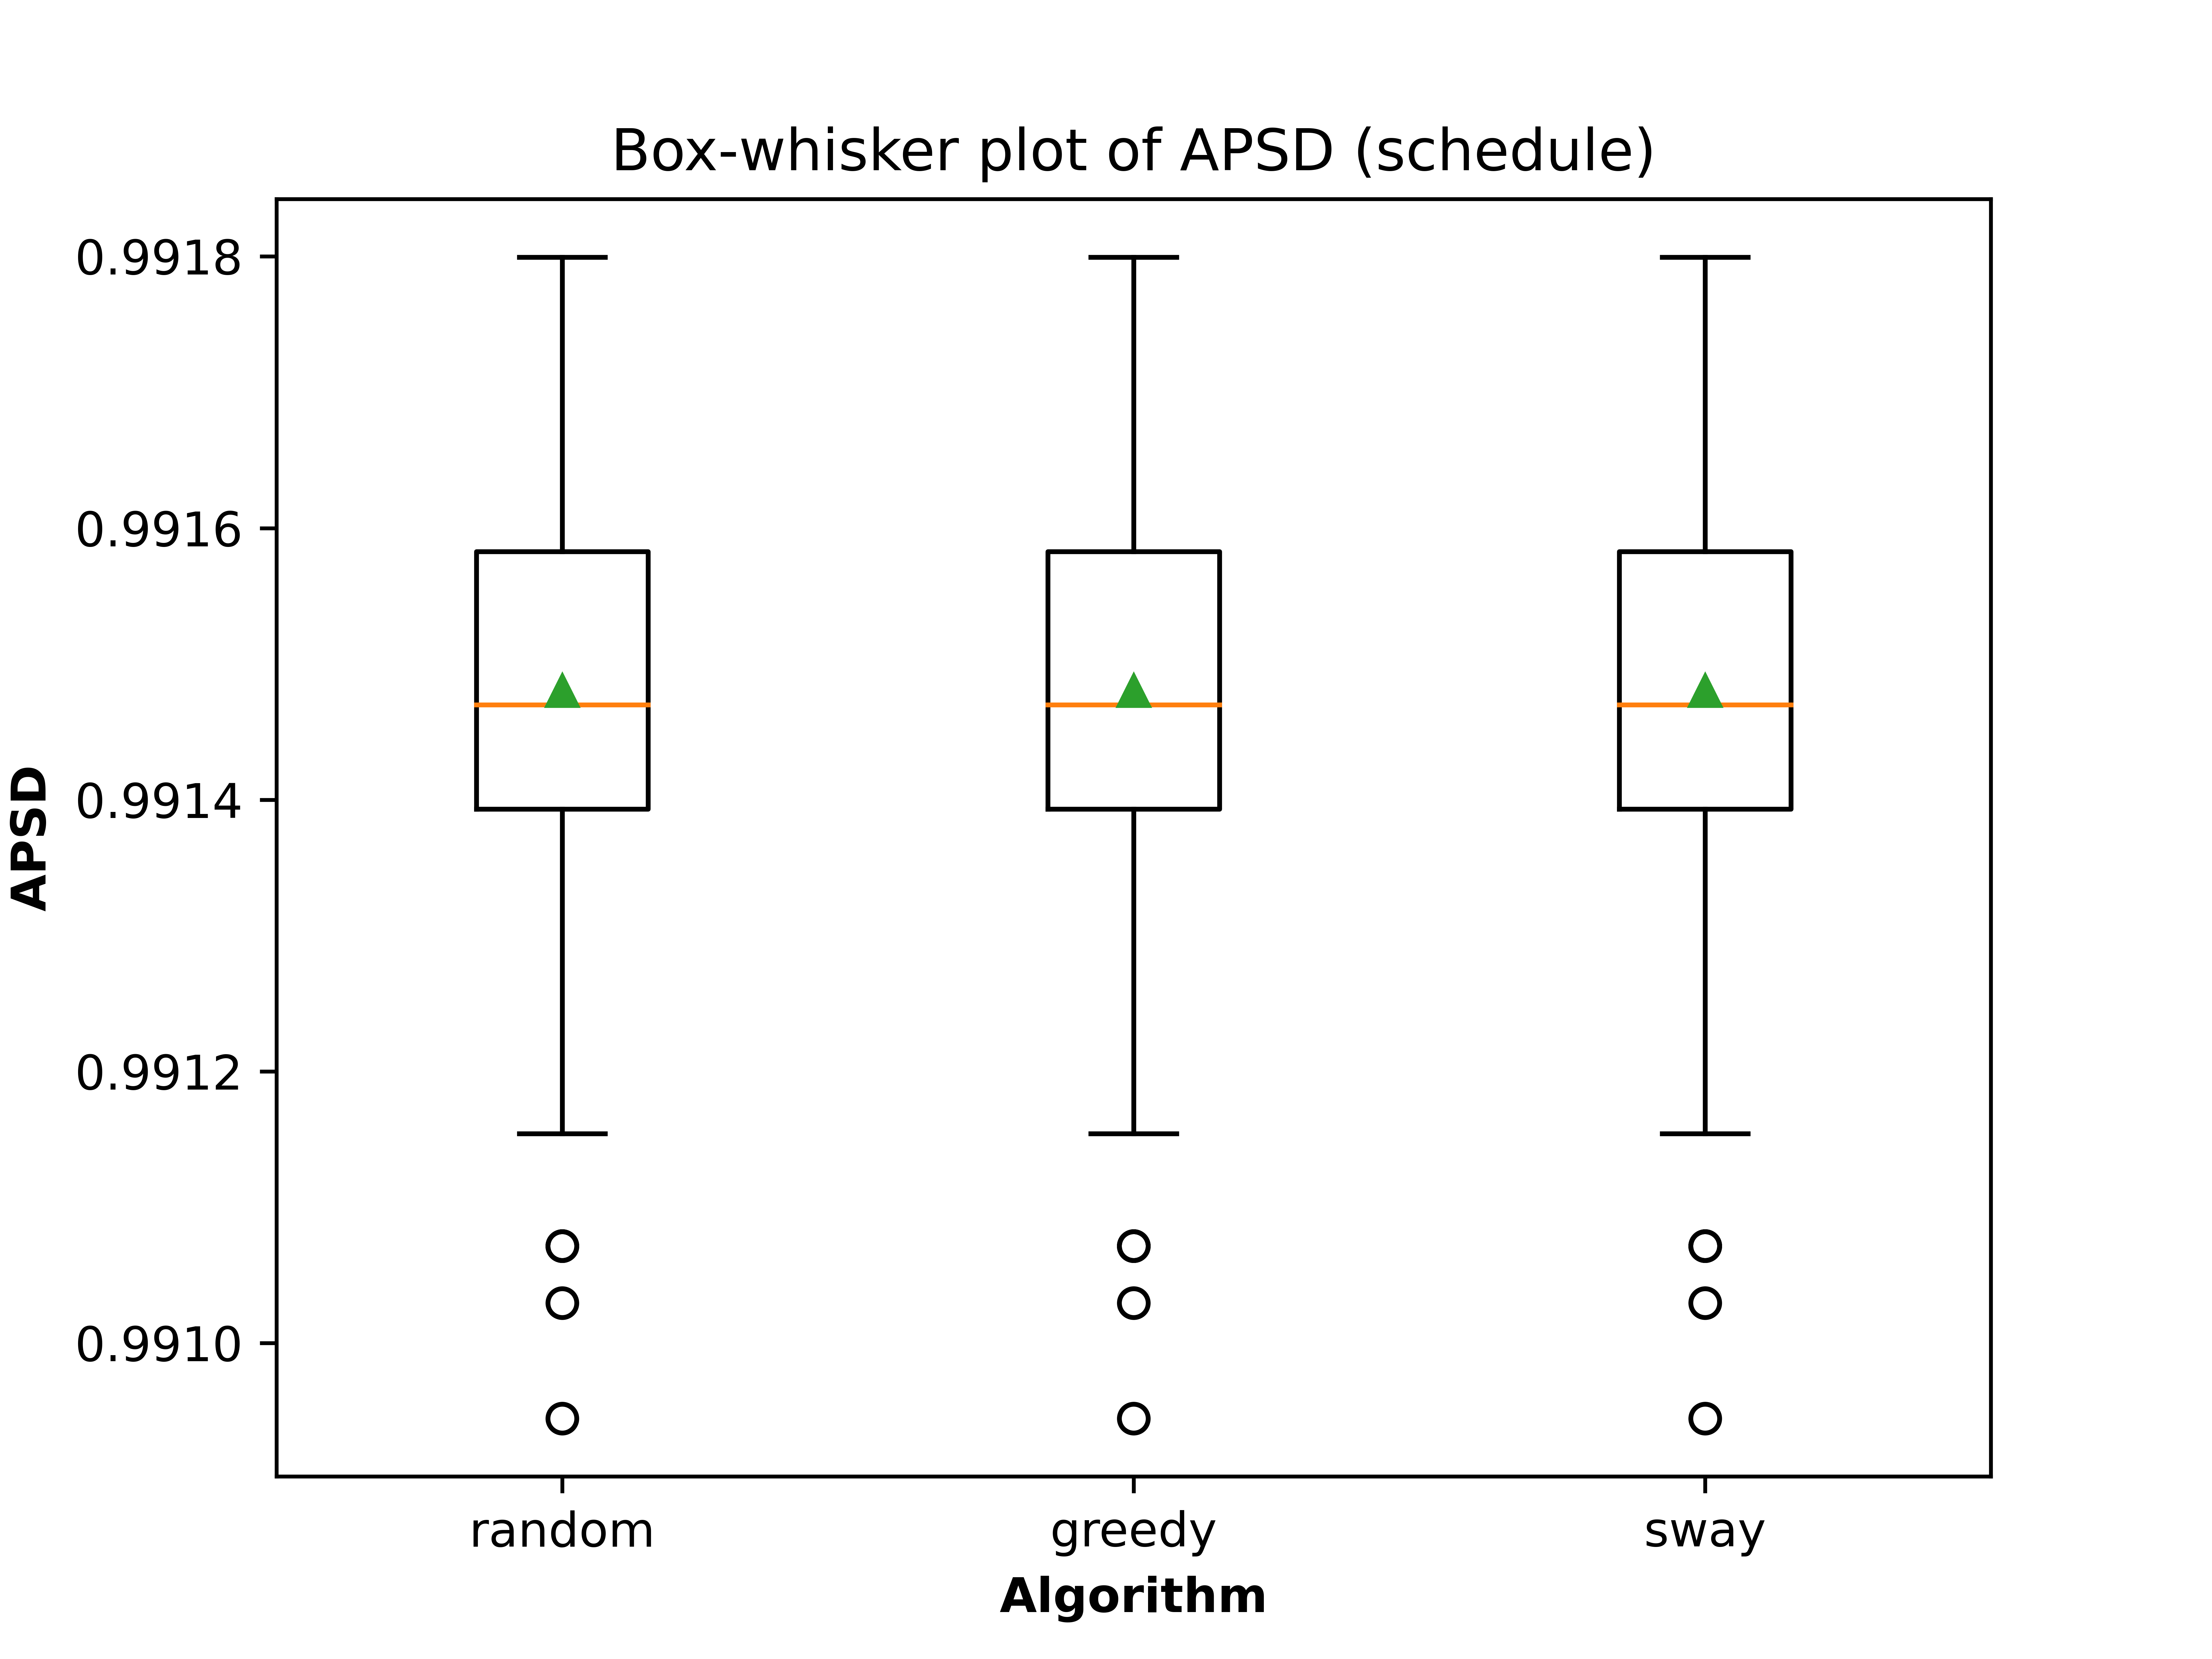
\includegraphics[width=\textwidth]{figures/APSD_schedule.png}
			\caption{{\bf schedule}, APSD}
		\end{subfigure}
		\hfill
		\begin{subfigure}[b]{0.4\linewidth}
			\centering
			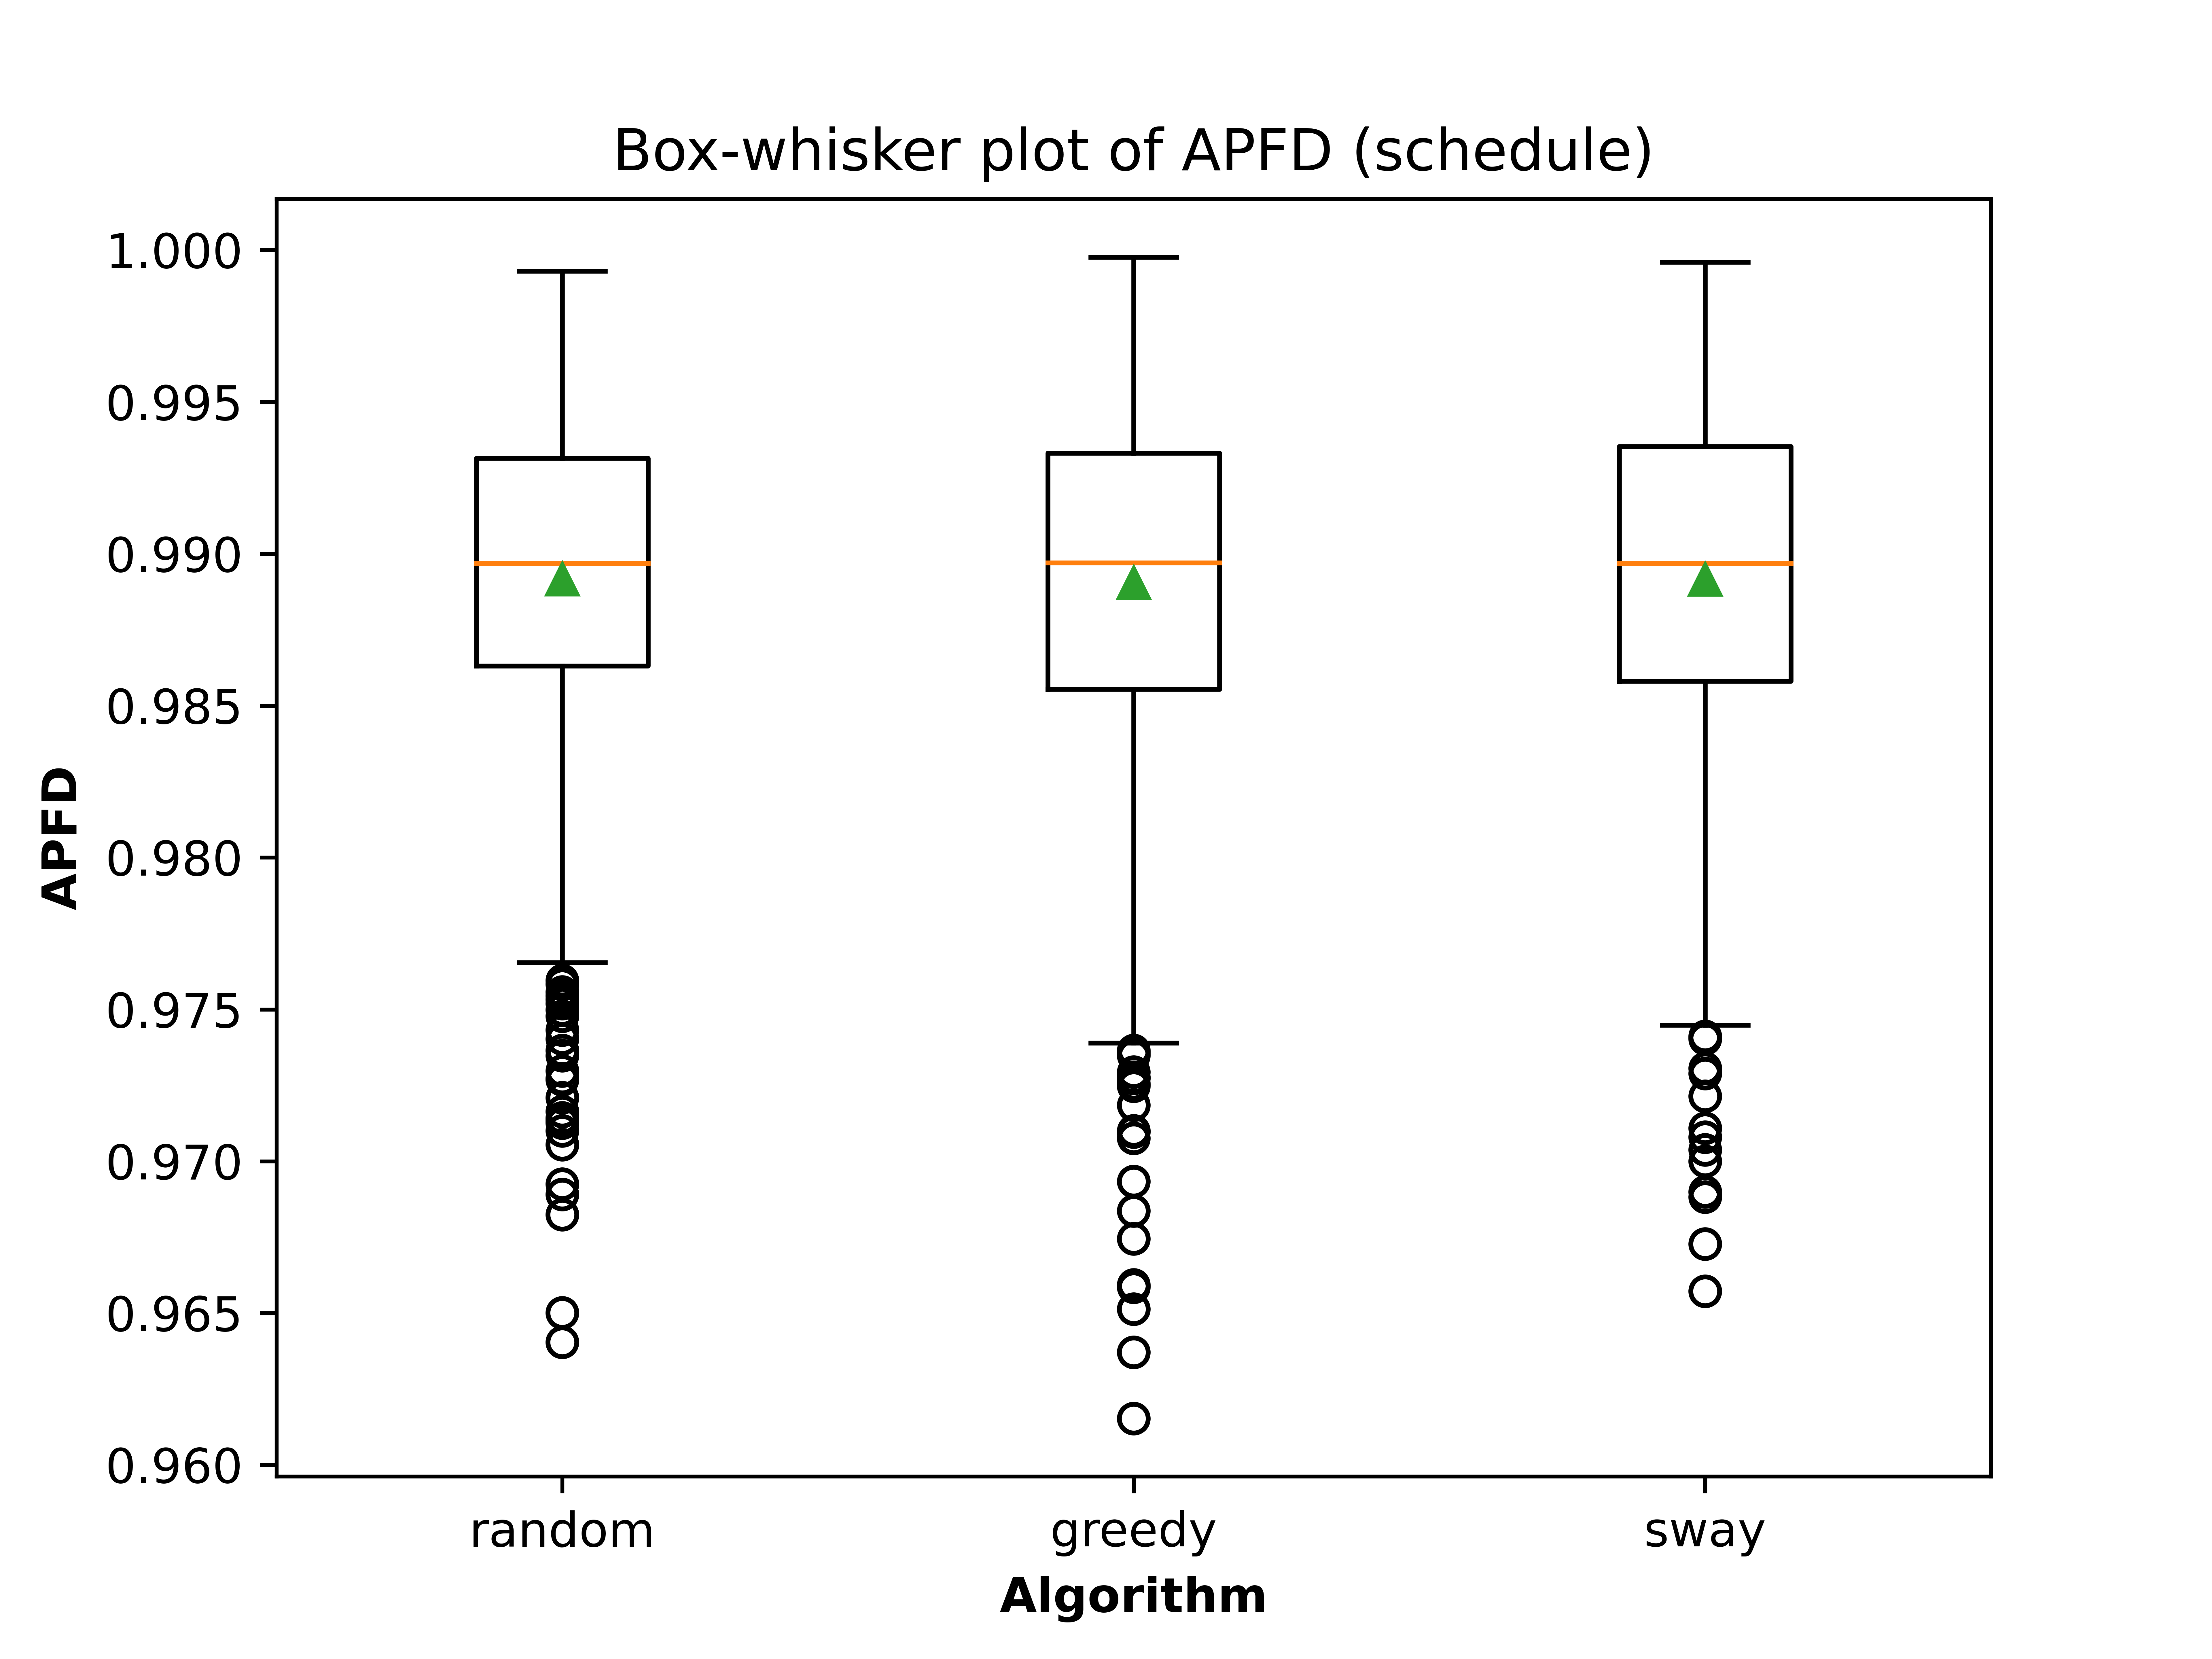
\includegraphics[width=\textwidth]{figures/APFD_schedule.png}
			\caption{{\bf schedule}, APFD}
		\end{subfigure}
		
		\vfill
		
		\begin{subfigure}[b]{0.4\linewidth}
			\centering
			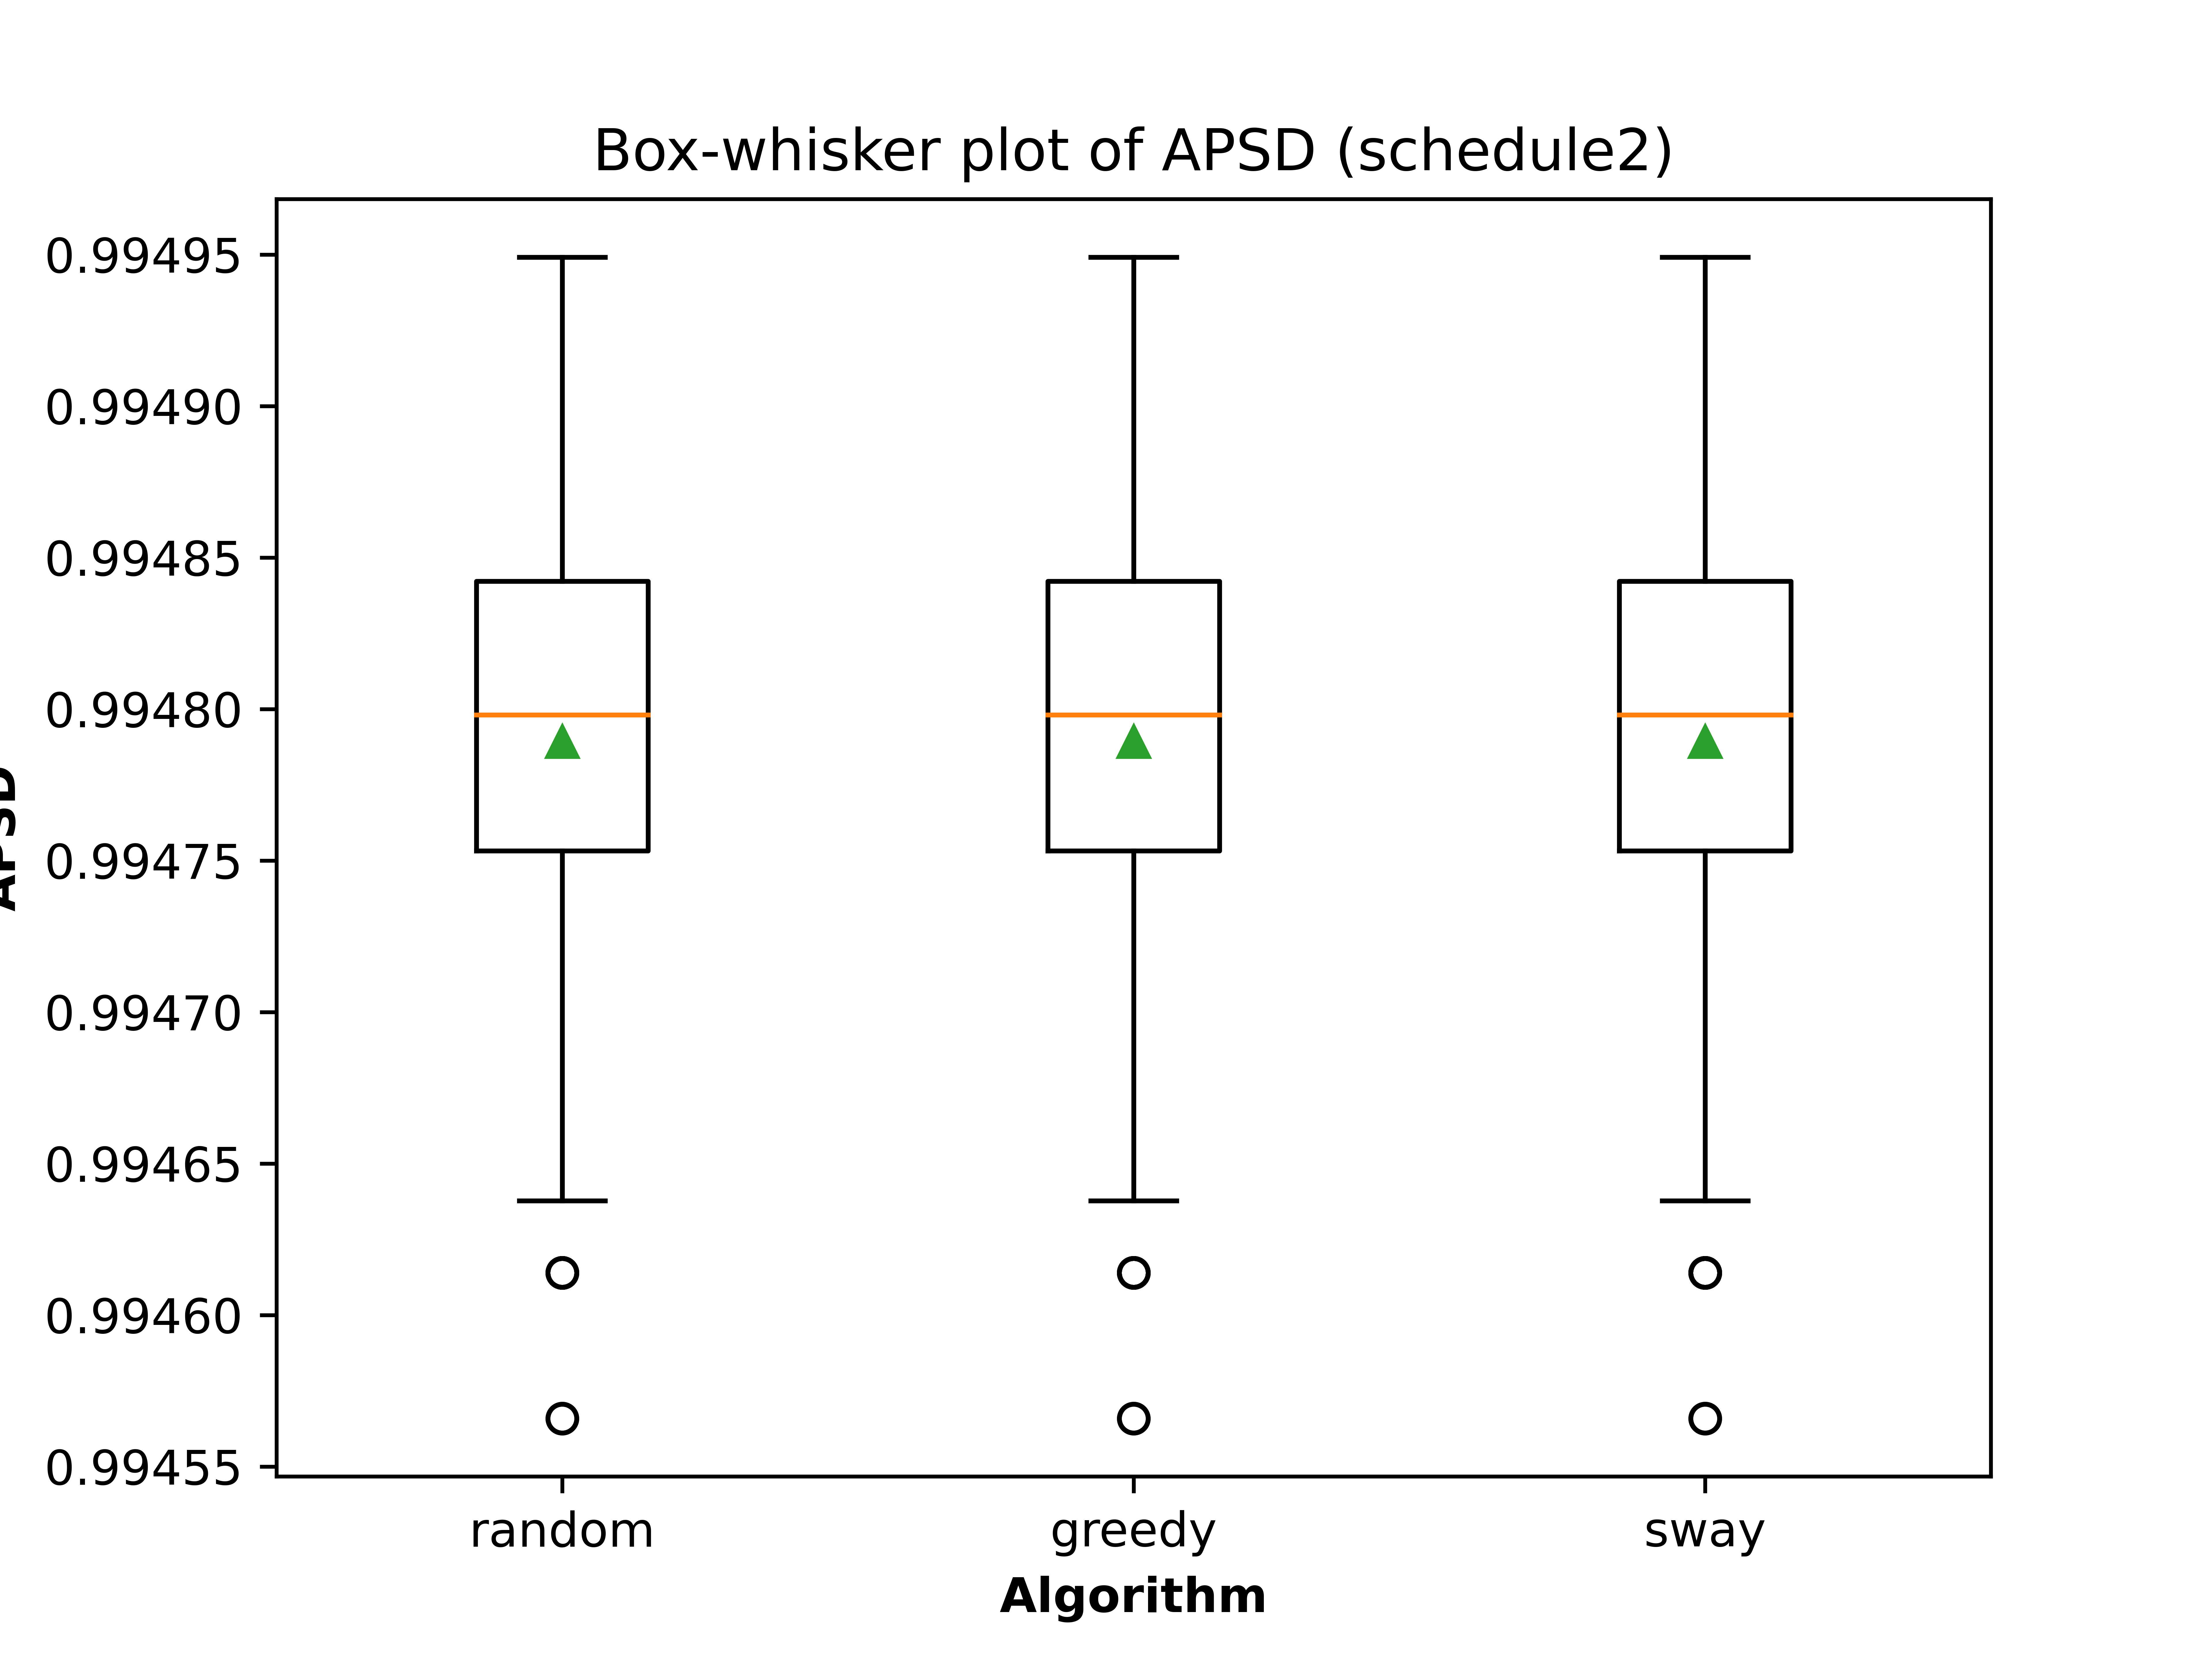
\includegraphics[width=\textwidth]{figures/APSD_schedule2.png}
			\caption{{\bf schedule2}, APSD}
		\end{subfigure}
		\hfill
		\begin{subfigure}[b]{0.4\linewidth}
			\centering
			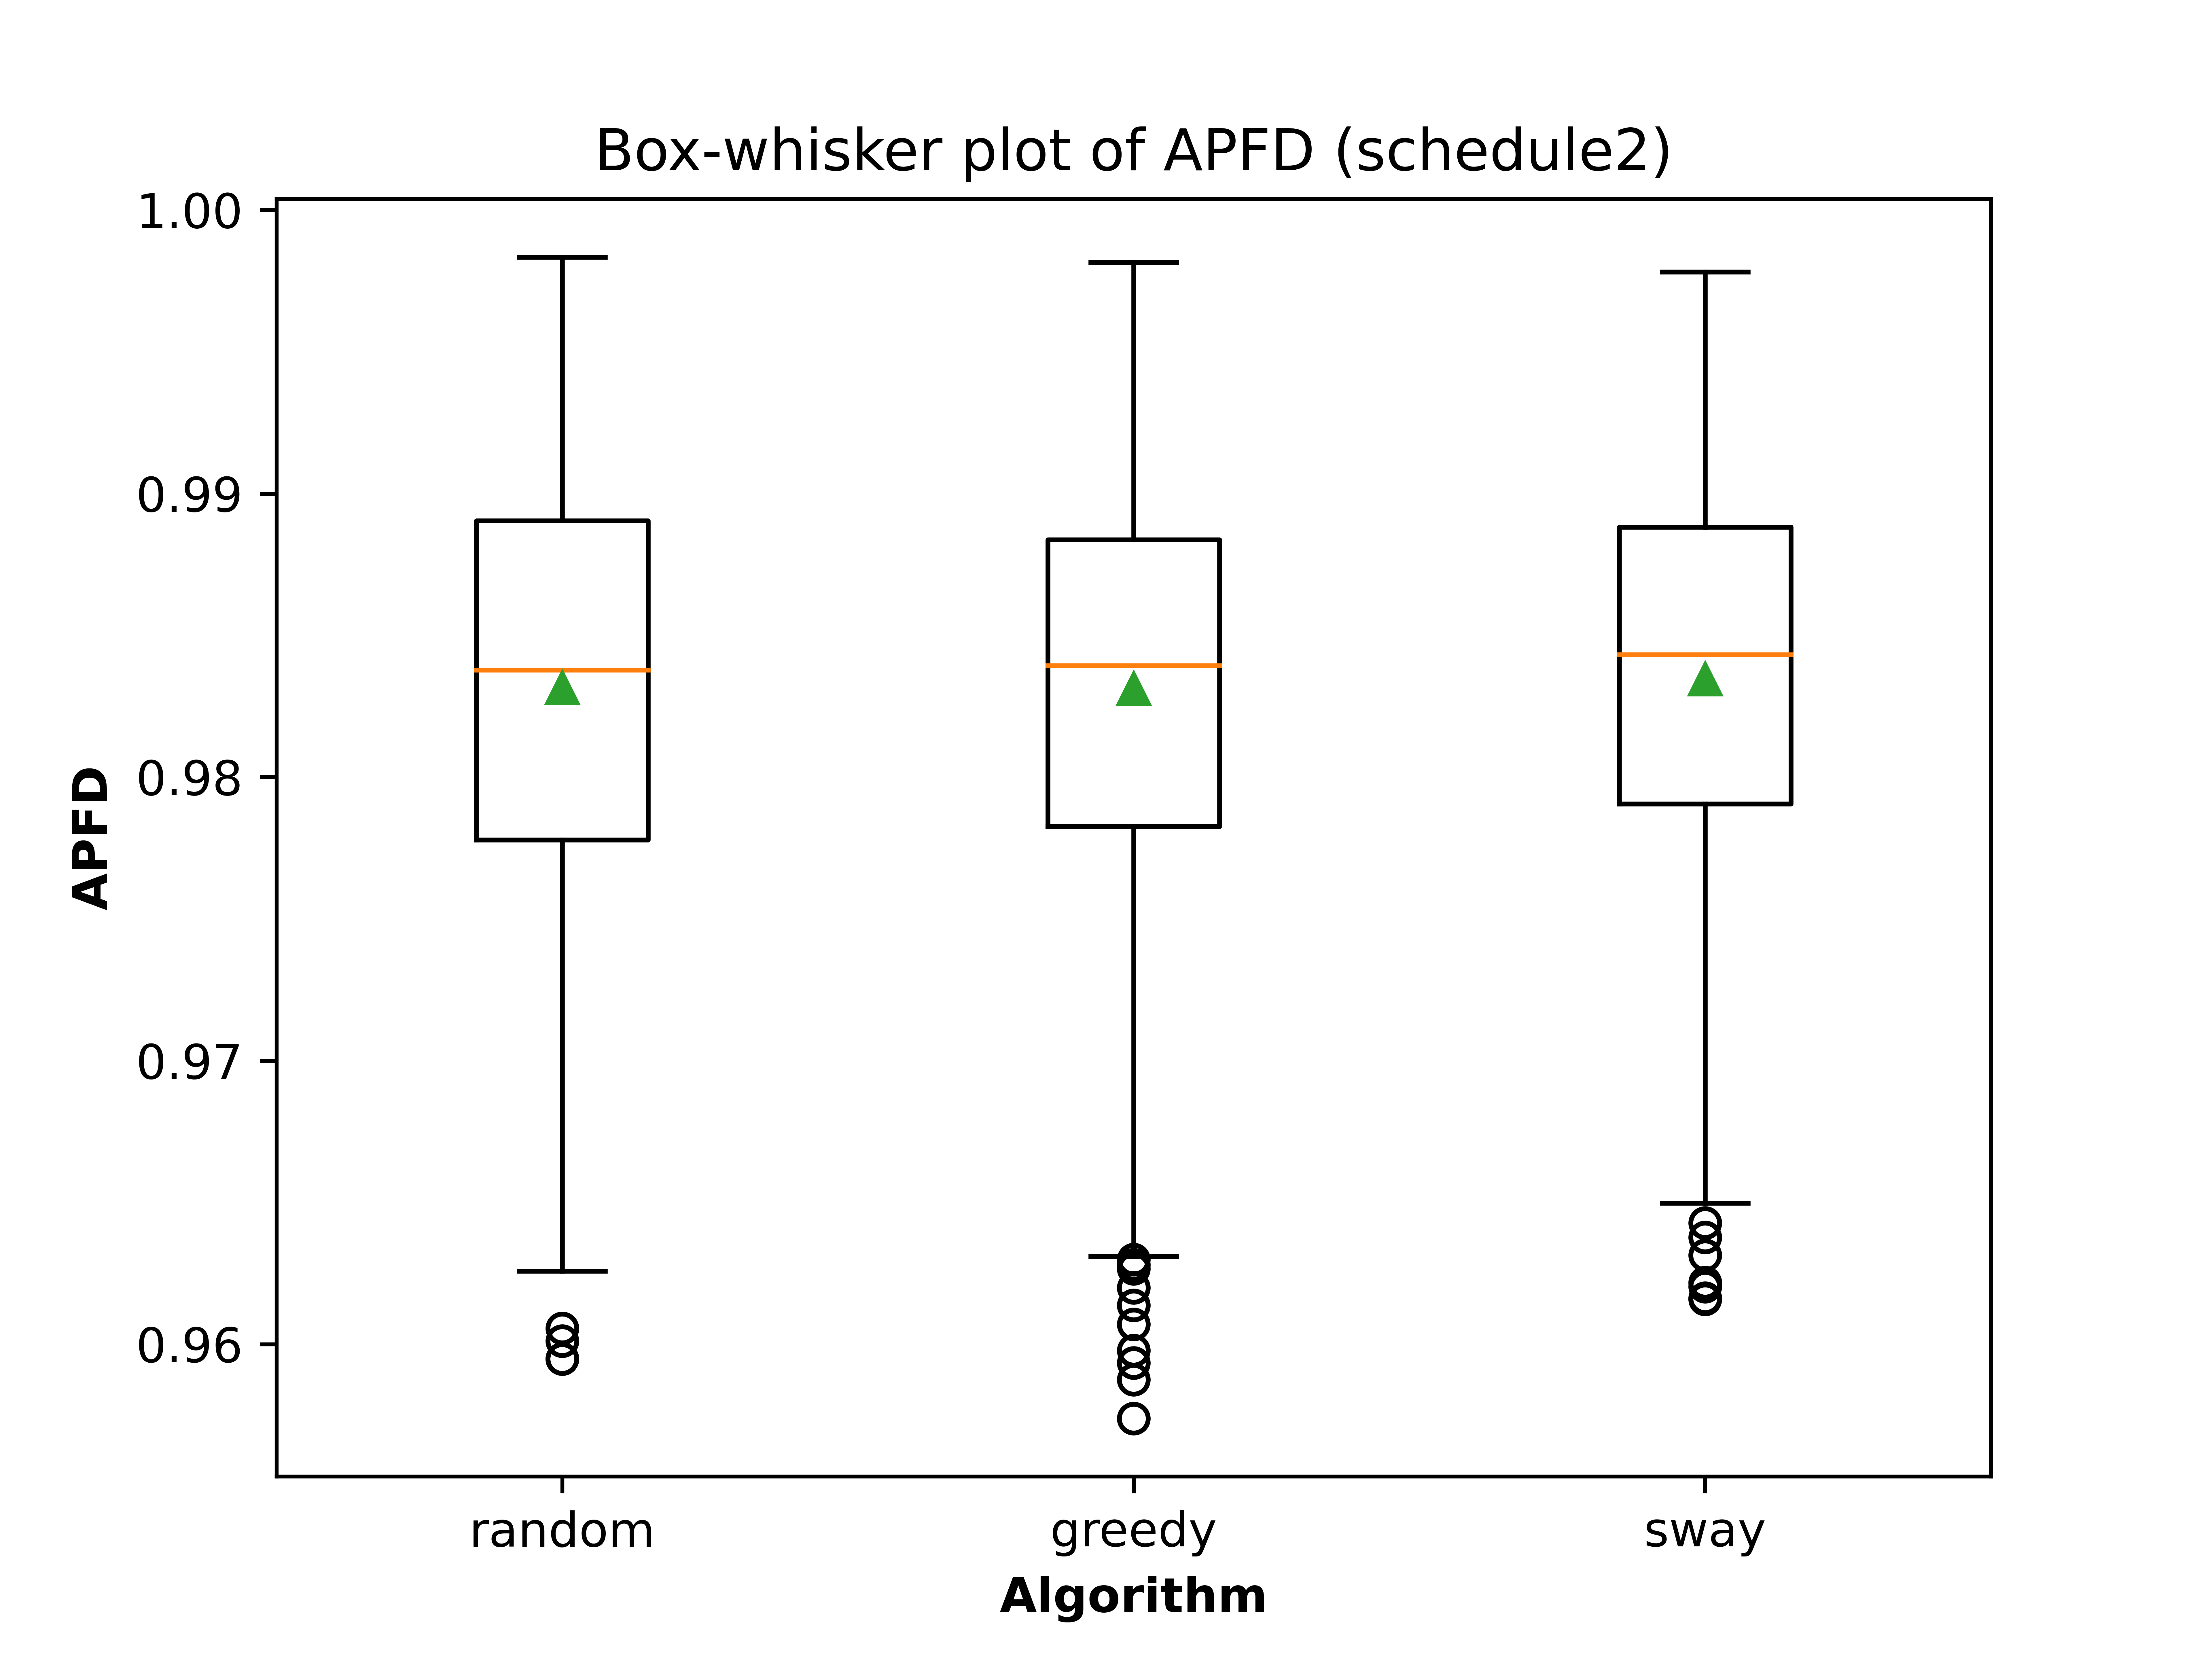
\includegraphics[width=\textwidth]{figures/APFD_schedule2.png}
			\caption{{\bf schedule2}, APFD}
		\end{subfigure}
		
		\caption{Comparison of APSD, APFD over three algorithms for {\bf schedule, schedule2}. (Beware of the scale! For instance, (c) and (d) have significantly different scales for the $y$-axis!)}
		\label{fig:main1}
	\end{figure*}
	
	\begin{figure*}
		\centering
		
		\begin{subfigure}[b]{0.4\linewidth}
			\centering
			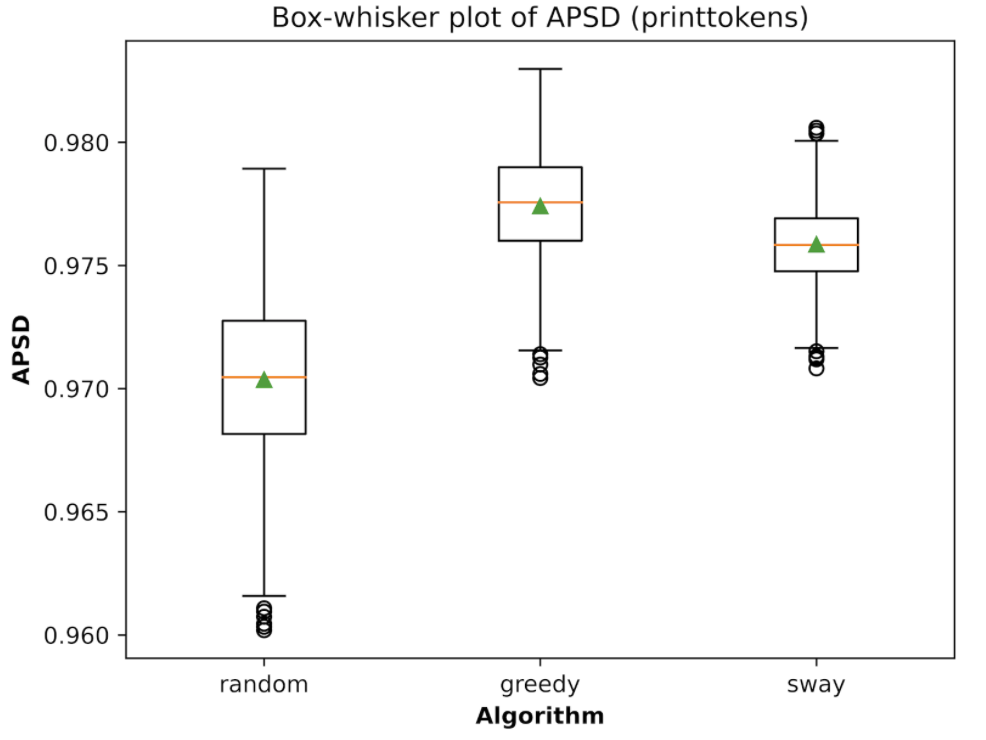
\includegraphics[width=\textwidth]{figures/APSD_printtokens.png}
			\caption{{\bf printtokens}, APSD}
		\end{subfigure}
		\hfill
		\begin{subfigure}[b]{0.4\linewidth}
			\centering
			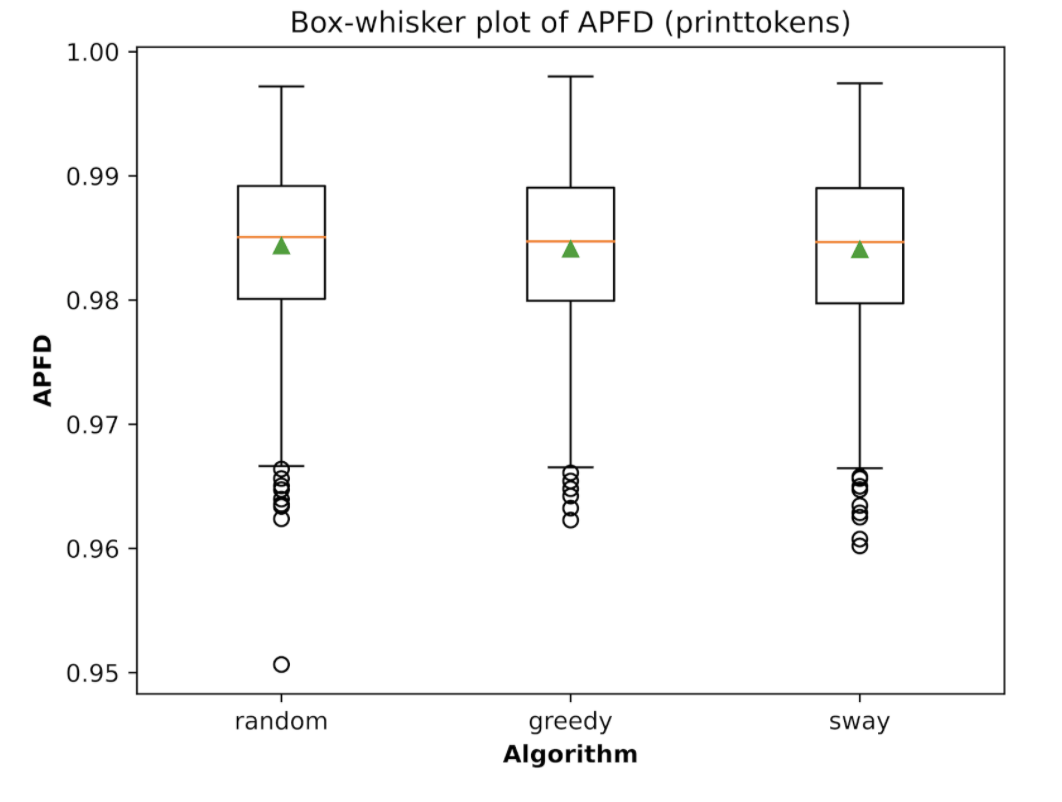
\includegraphics[width=\textwidth]{figures/APFD_printtokens.png}
			\caption{{\bf printtokens}, APFD}
		\end{subfigure}
		
		\vfill
		
		\begin{subfigure}[b]{0.4\linewidth}
			\centering
			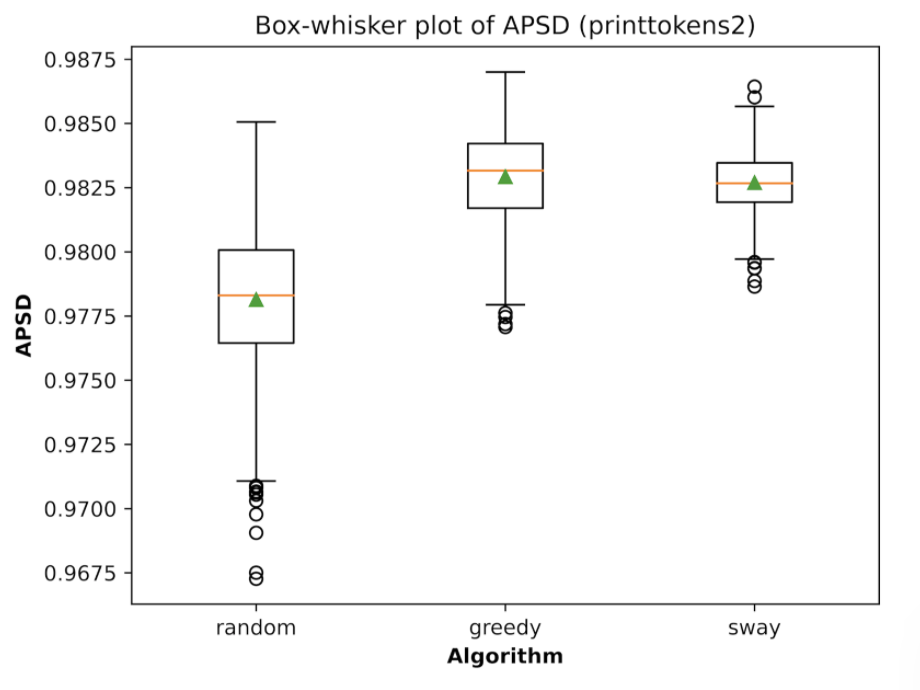
\includegraphics[width=\textwidth]{figures/APSD_printtokens2.png}
			\caption{{\bf printtokens2}, APSD}
		\end{subfigure}
		\hfill
		\begin{subfigure}[b]{0.4\linewidth}
			\centering
			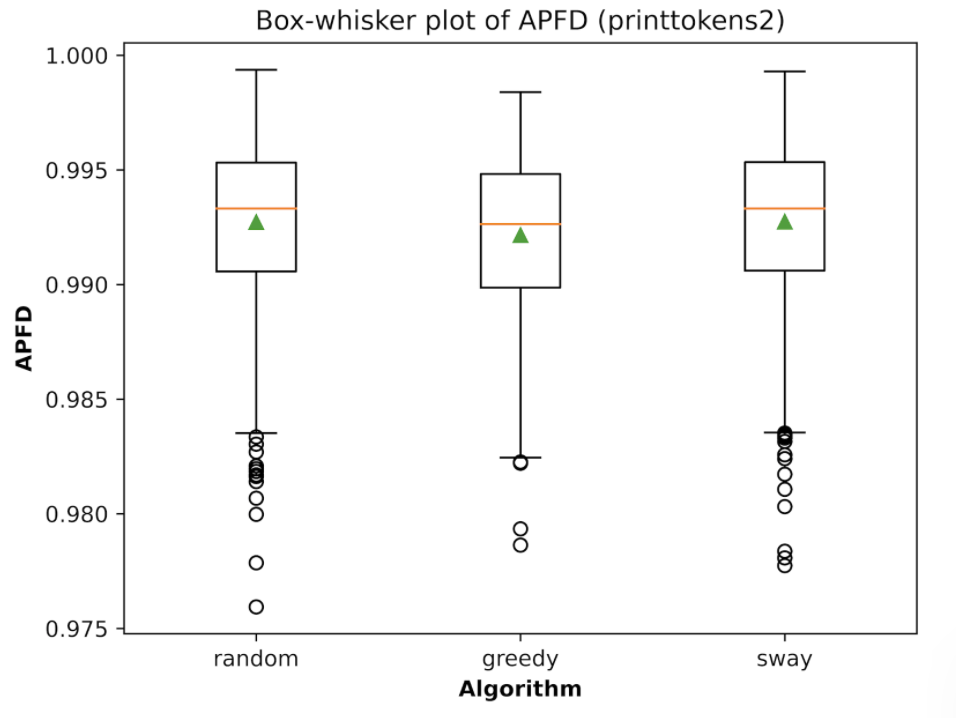
\includegraphics[width=\textwidth]{figures/APFD_printtokens2.png}
			\caption{{\bf printtokens2}, APFD}
		\end{subfigure}
		
		\caption{Comparison of APSD, APFD over three algorithms for {\bf printtokens, printtokens2}.}
		\label{fig:main2}
	\end{figure*}
	
	\begin{figure*}
		\centering
		
		\begin{subfigure}[b]{0.4\linewidth}
			\centering
			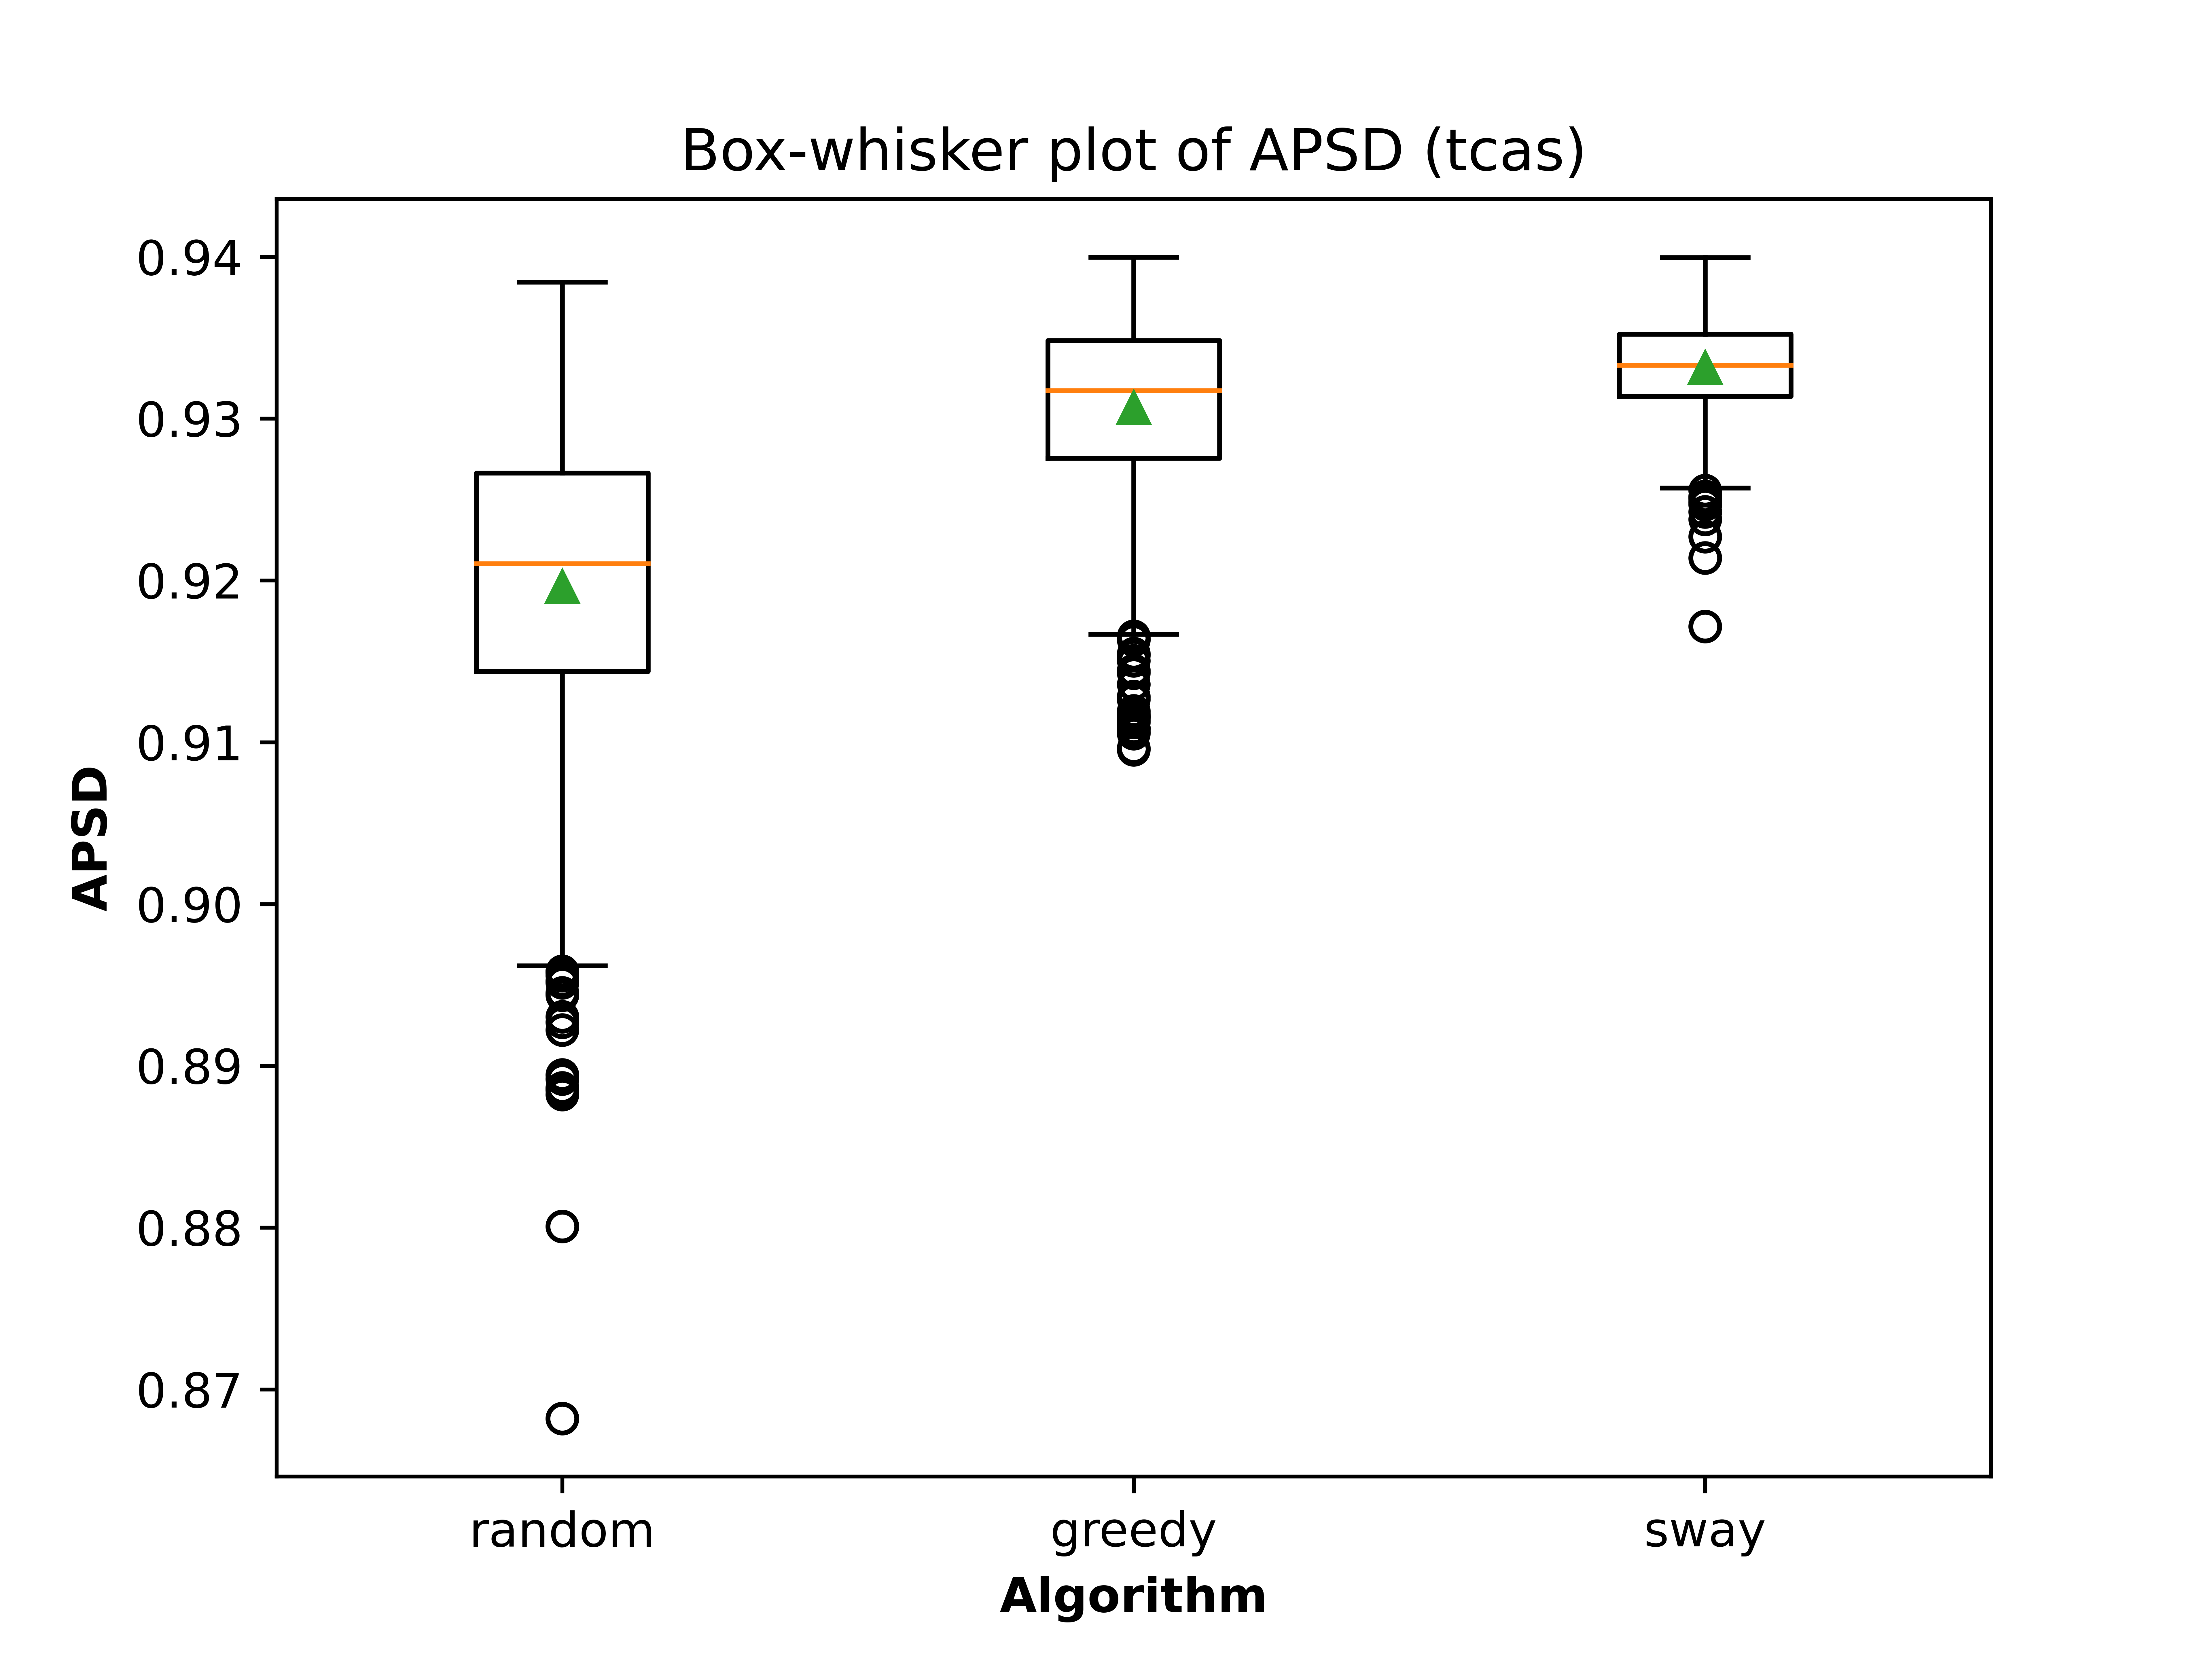
\includegraphics[width=\textwidth]{figures/APSD_tcas.png}
			\caption{{\bf tcas}, APSD}
		\end{subfigure}
		\hfill
		\begin{subfigure}[b]{0.4\linewidth}
			\centering
			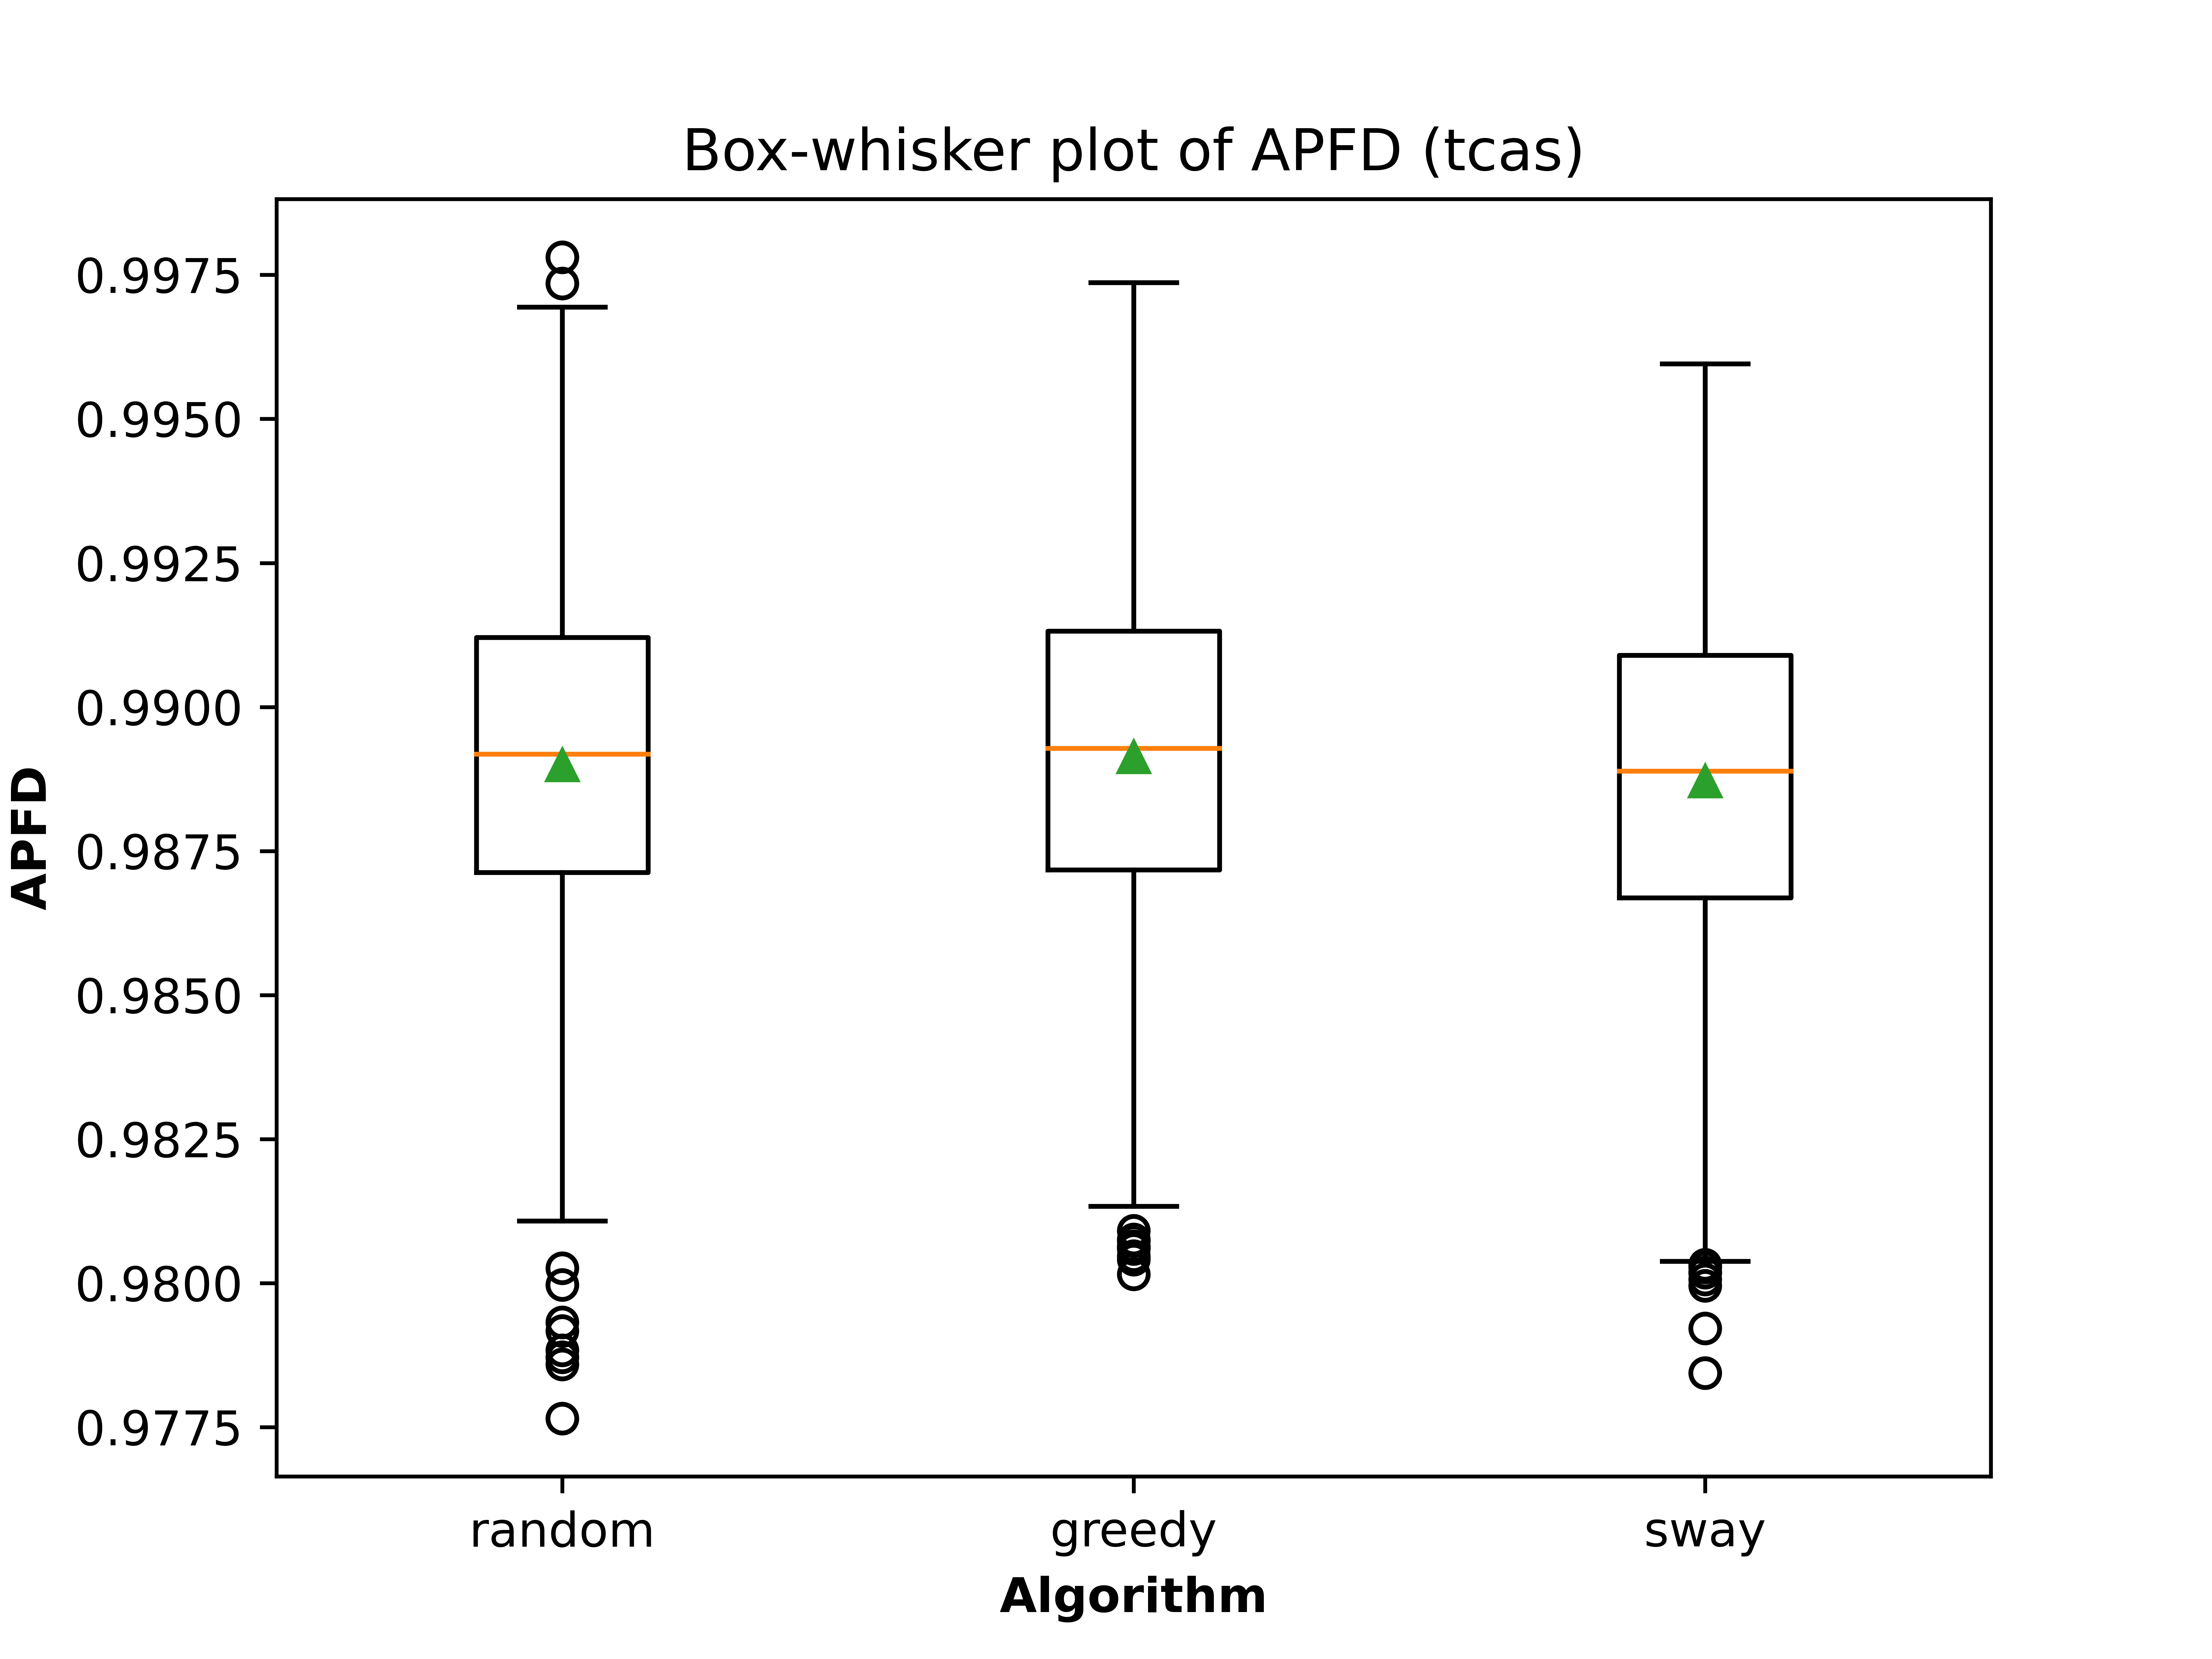
\includegraphics[width=\textwidth]{figures/APFD_tcas.png}
			\caption{{\bf tcas}, APFD}
		\end{subfigure}
		
		\vfill
		
		\begin{subfigure}[b]{0.4\linewidth}
			\centering
			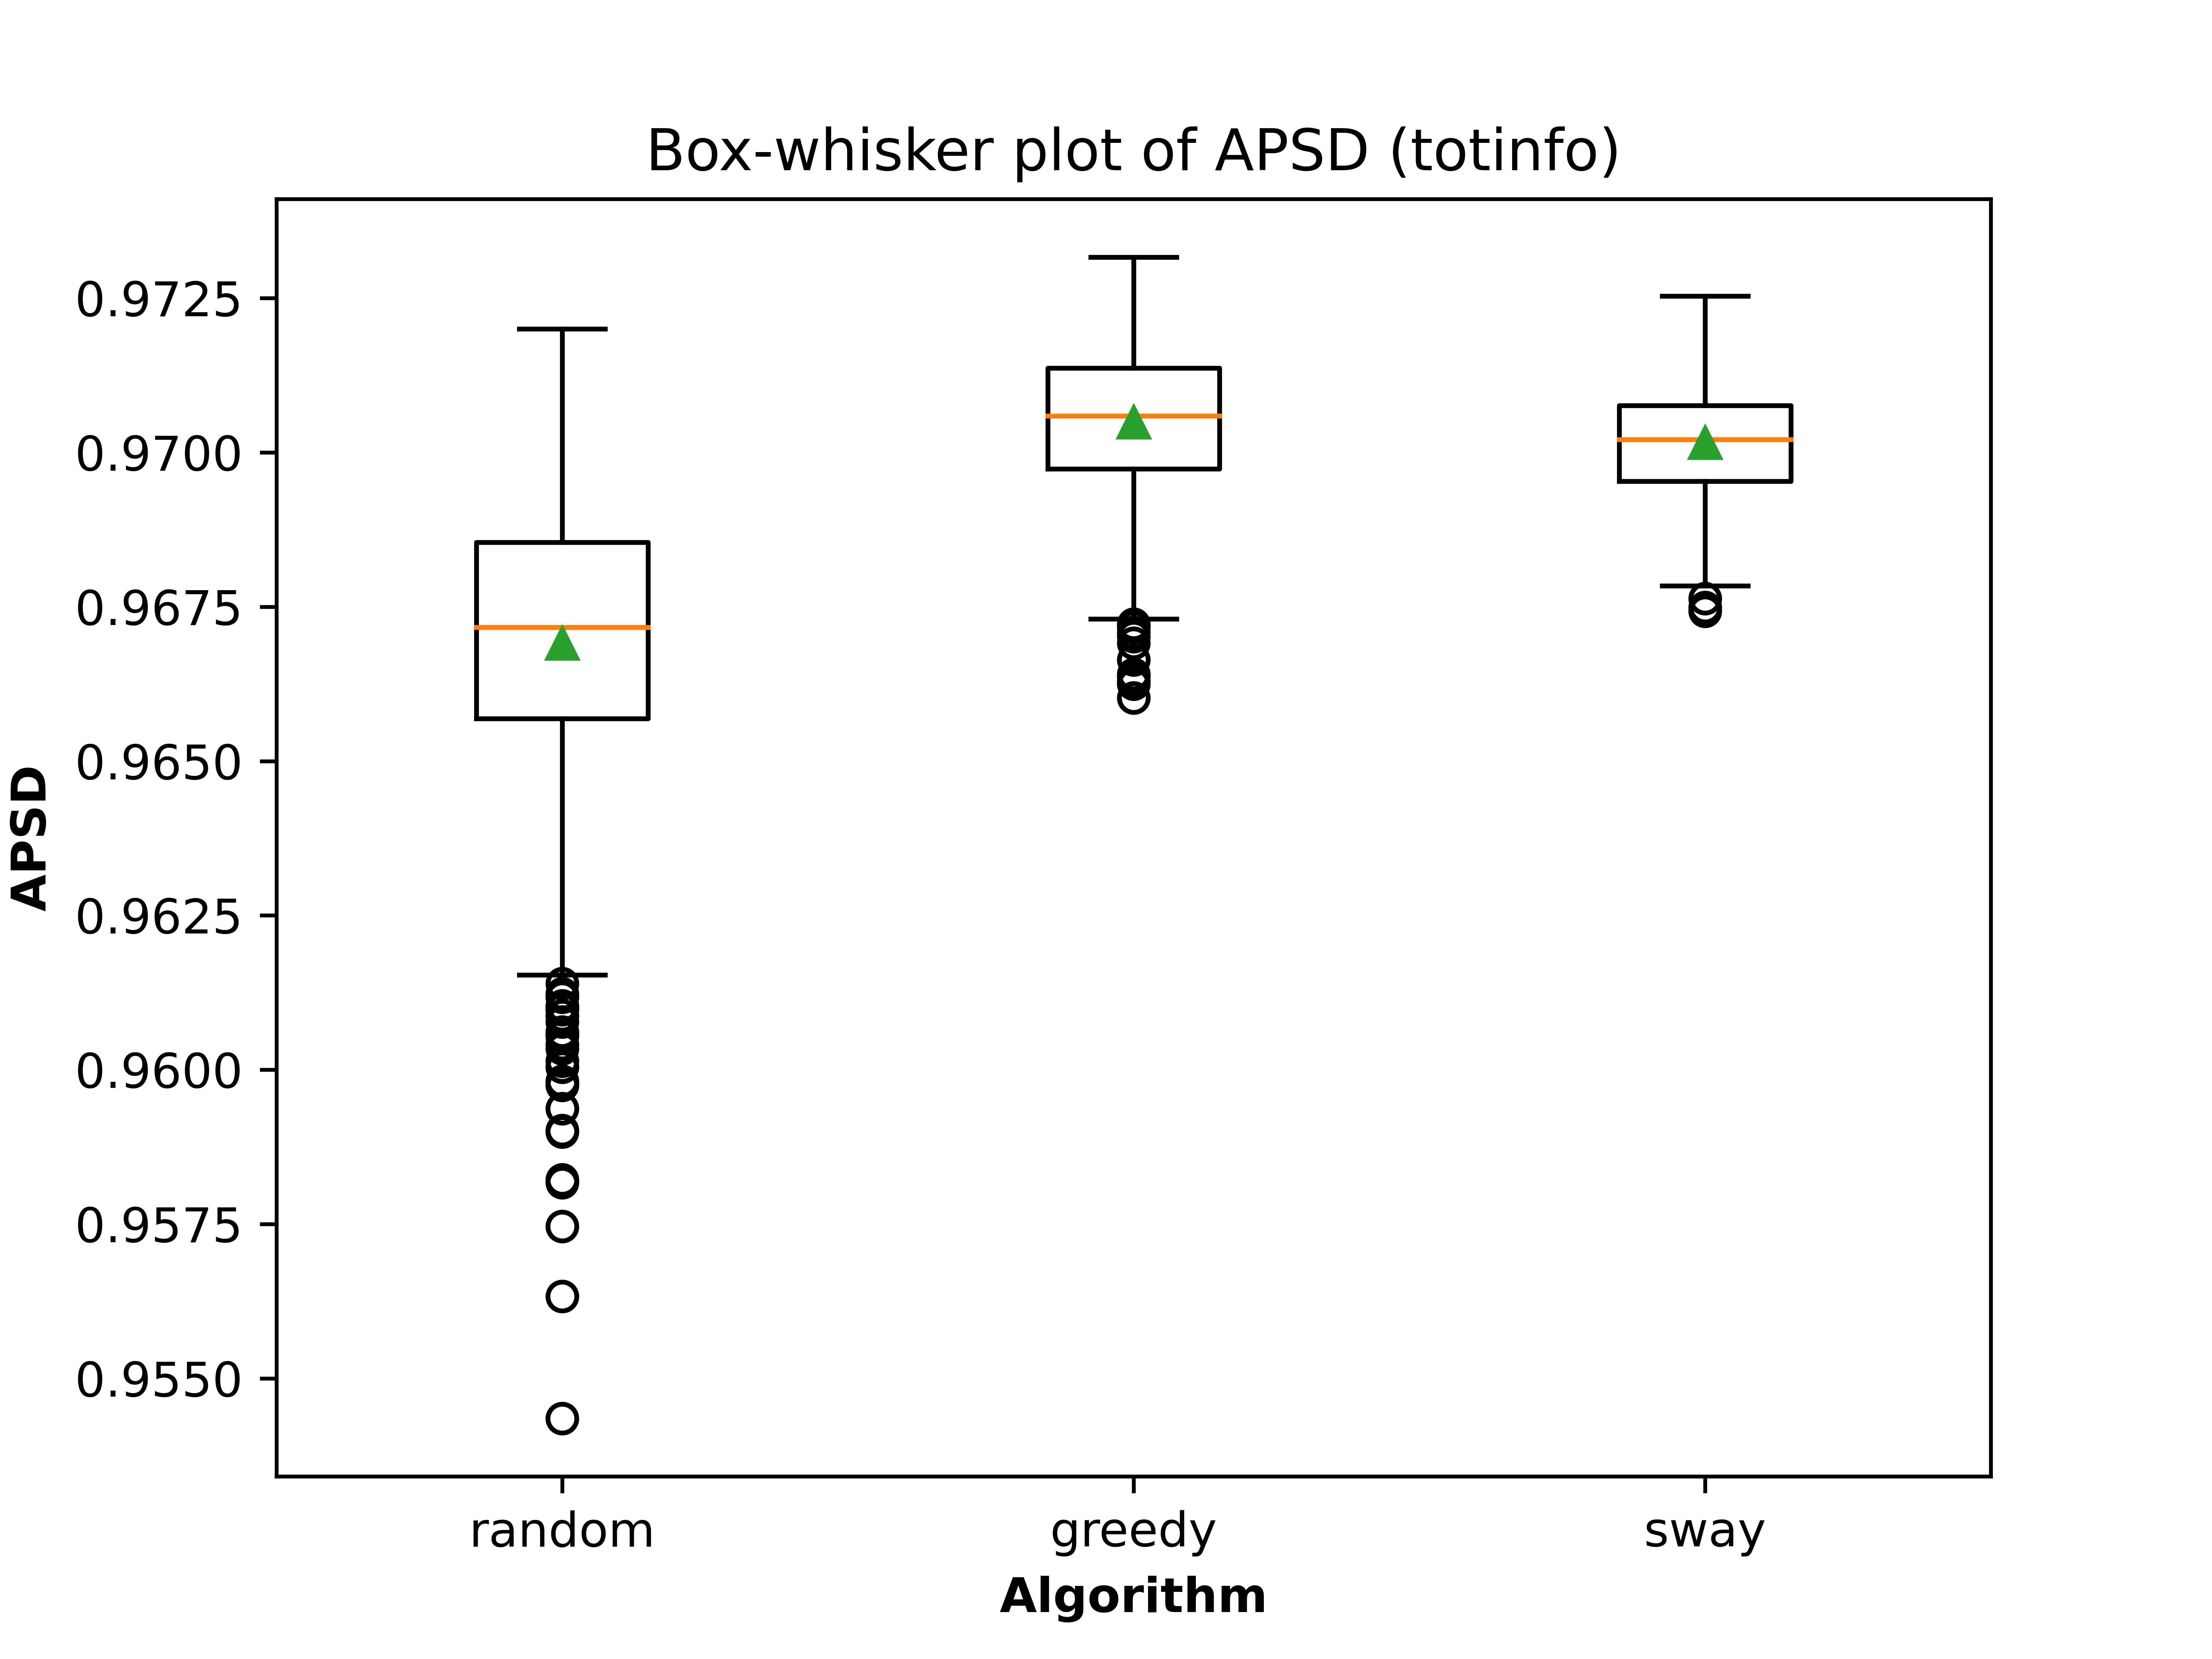
\includegraphics[width=\textwidth]{figures/APSD_totinfo.png}
			\caption{{\bf totinfo}, APSD}
		\end{subfigure}
		\hfill
		\begin{subfigure}[b]{0.4\linewidth}
			\centering
			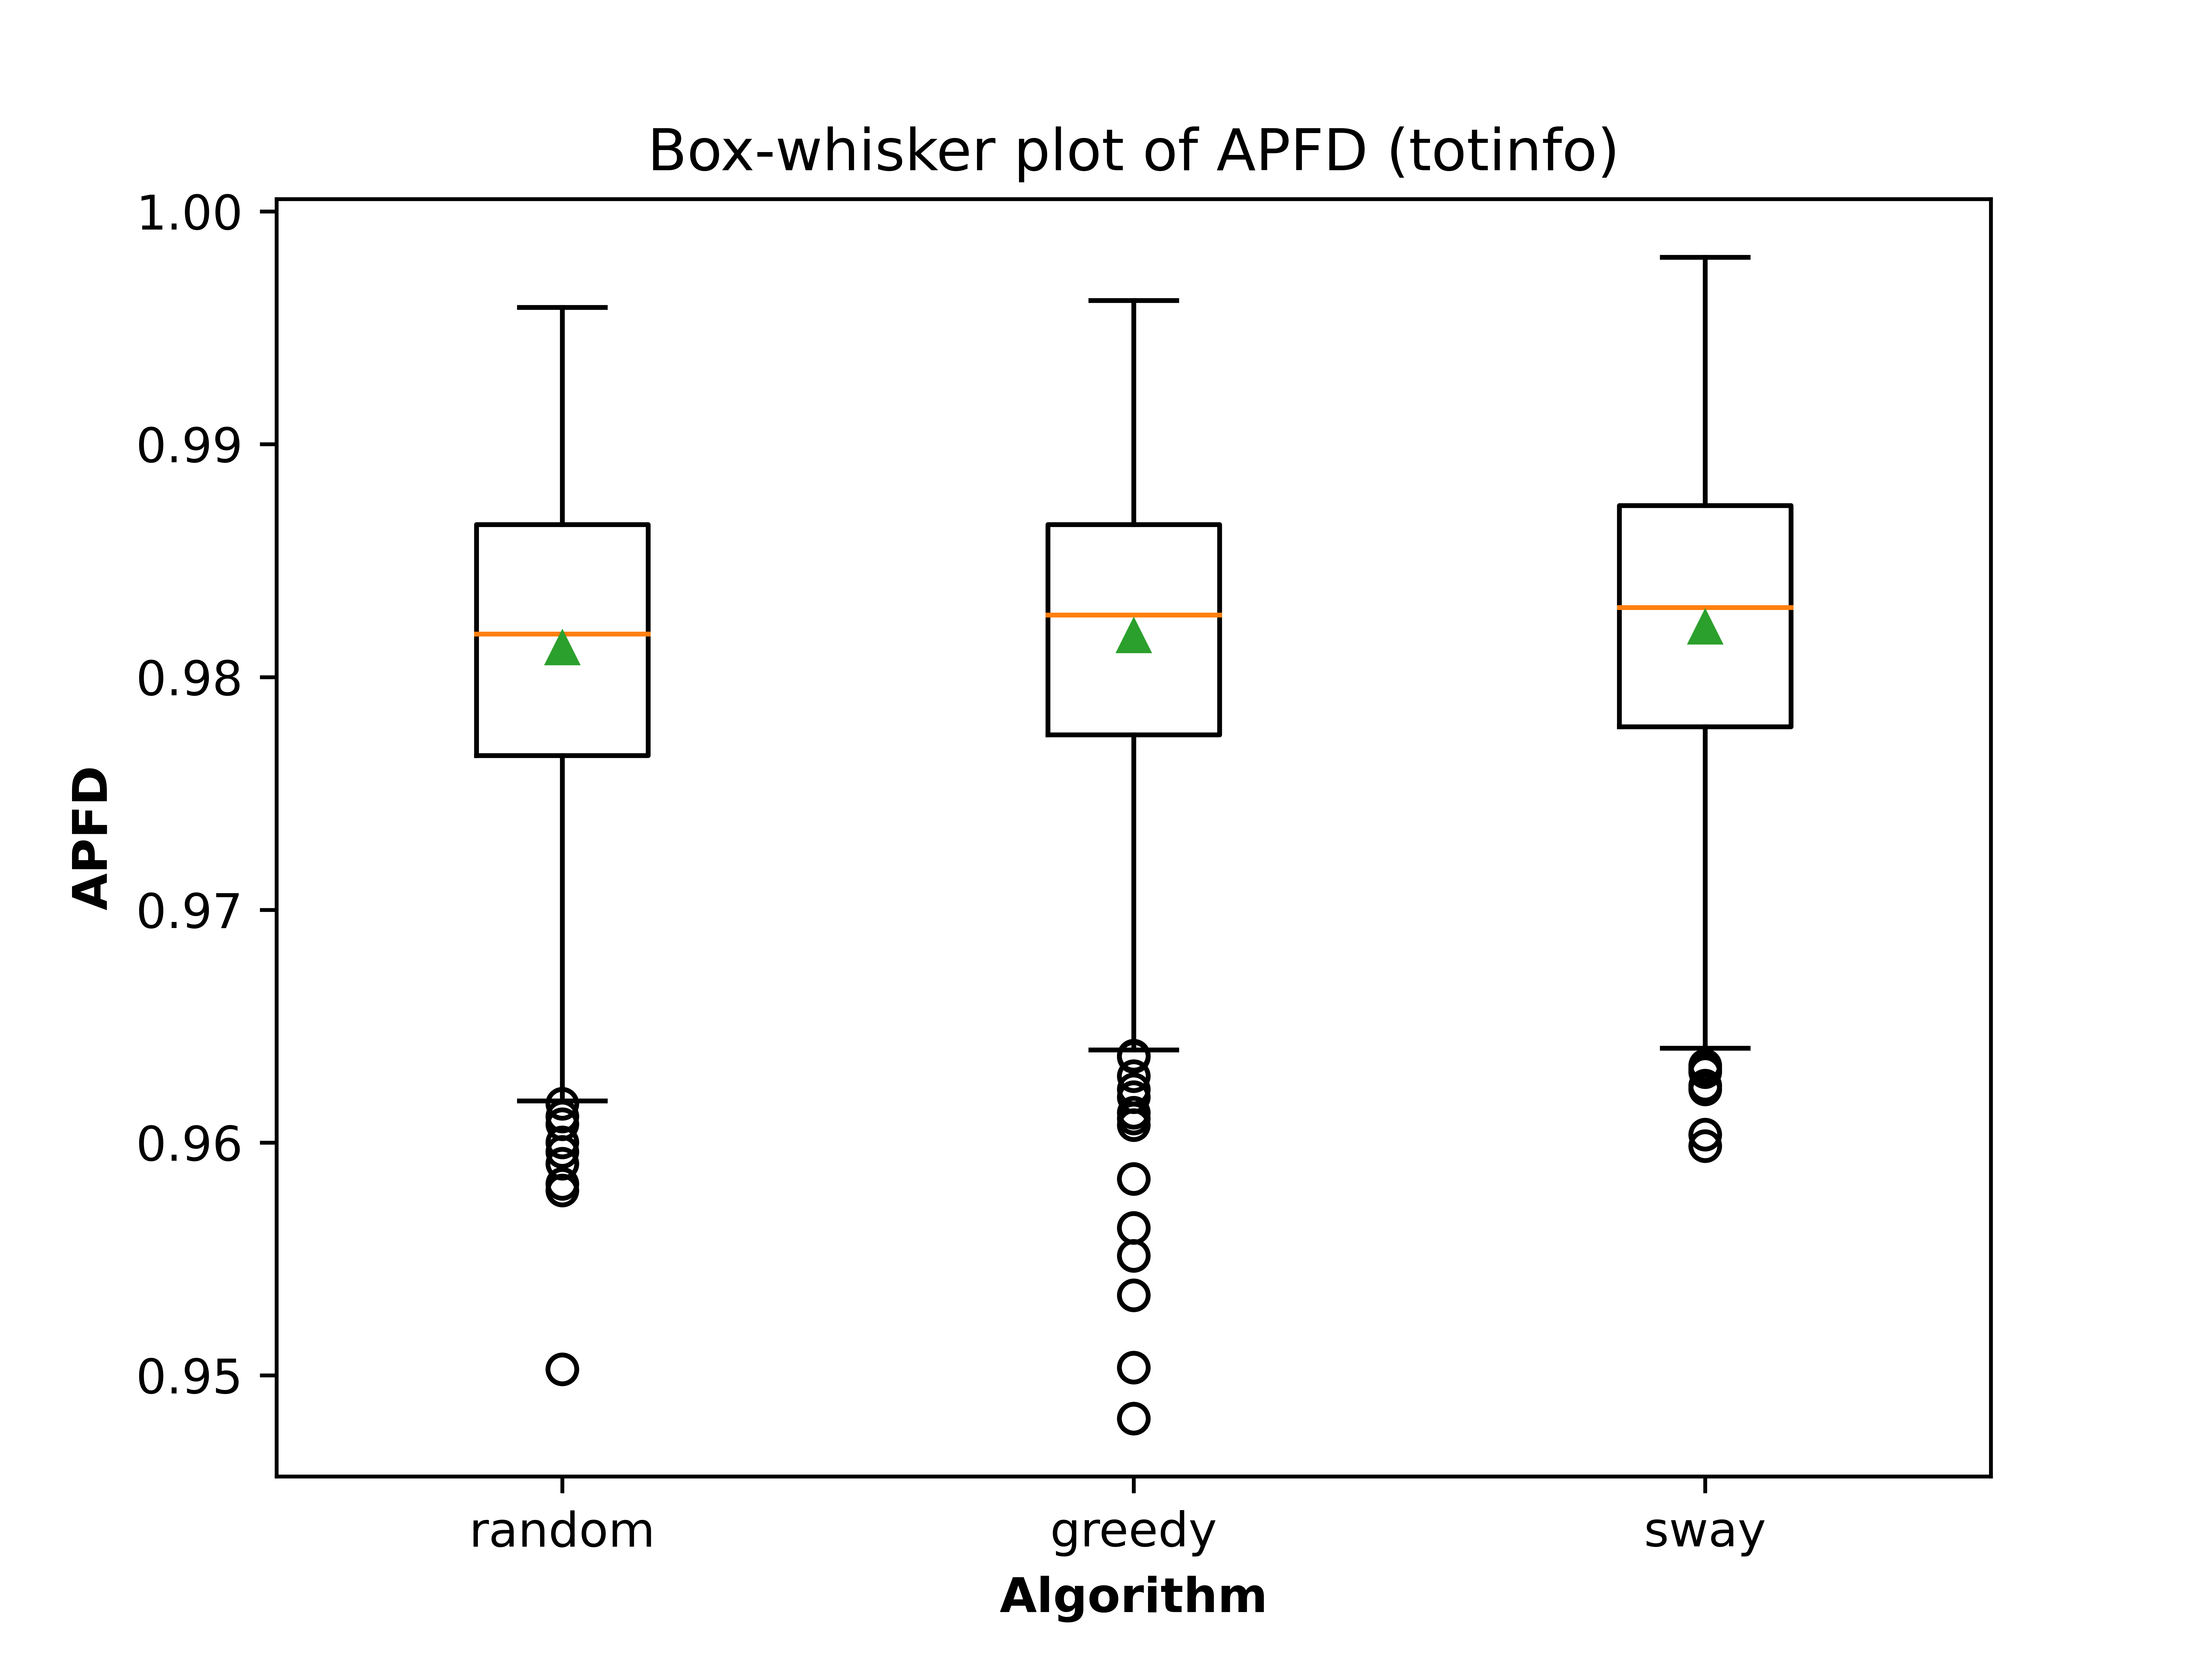
\includegraphics[width=\textwidth]{figures/APFD_totinfo.png}
			\caption{{\bf totinfo}, APFD}
		\end{subfigure}
		
		\caption{Comparison of APSD, APFD over three algorithms for {\bf tcas, totinfo}.}
		\label{fig:main3}
	\end{figure*}
	
	
	\begin{figure*}
		\centering
		\begin{subfigure}[b]{0.4\linewidth}
			\centering
			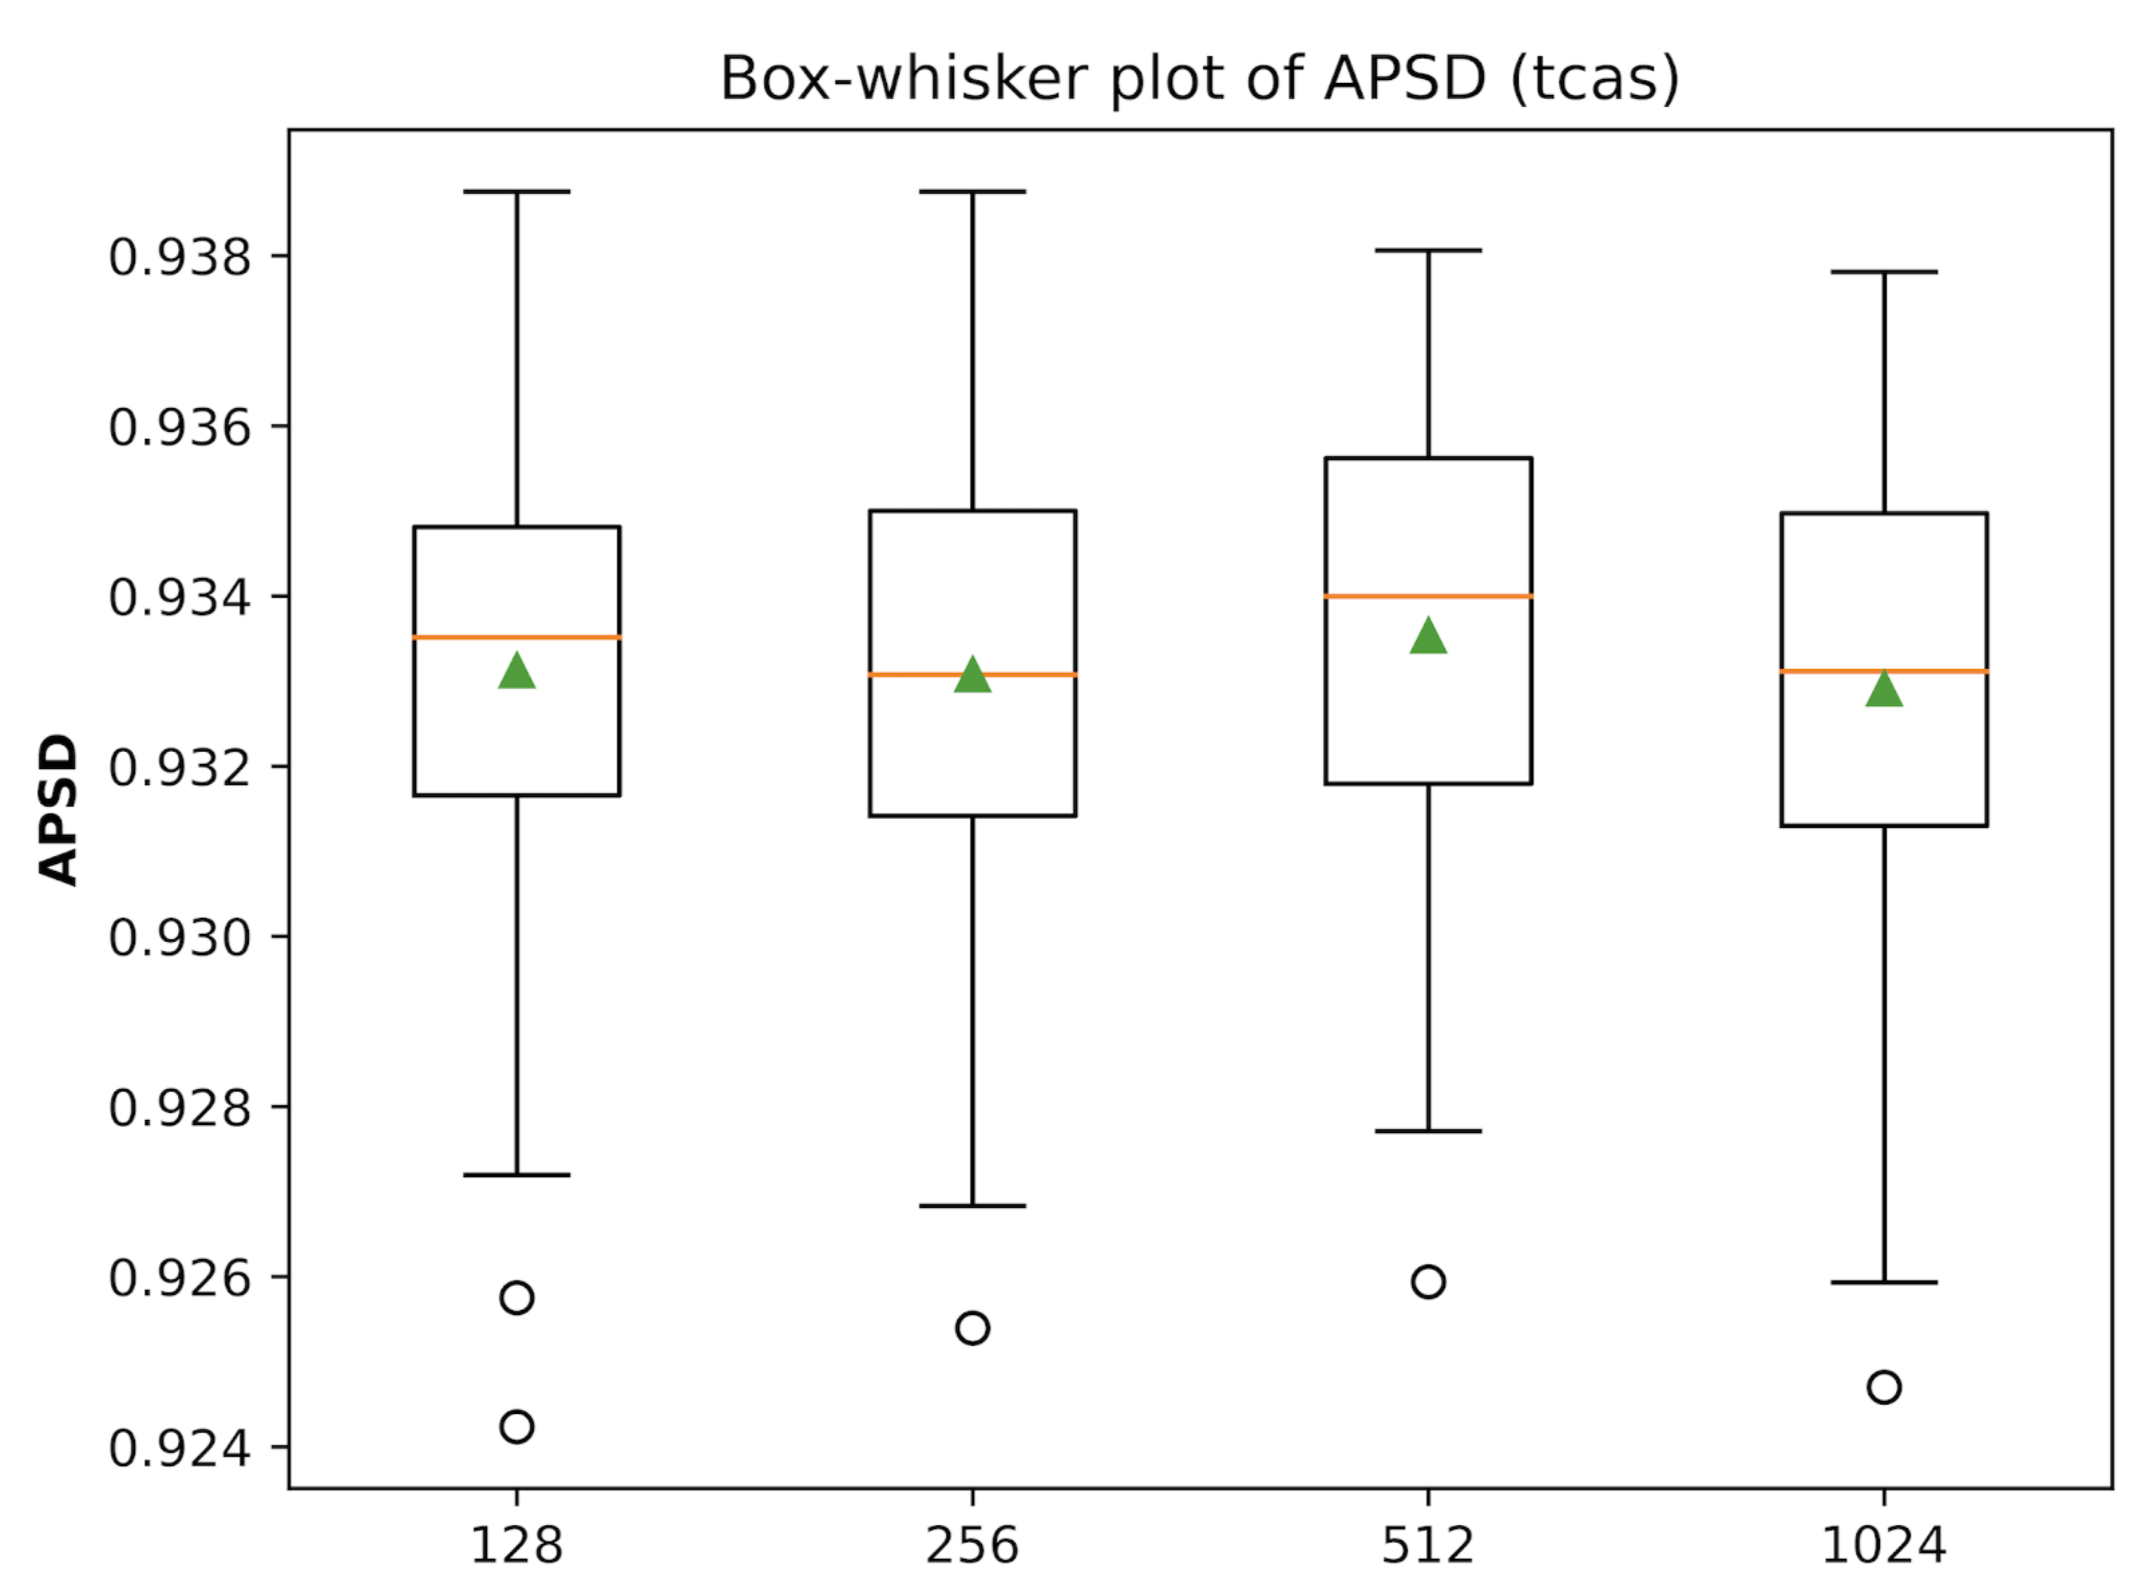
\includegraphics[width=\textwidth]{hyperparam/apsd.png}
			\caption{APSD}
		\end{subfigure}
		\hfill
		\begin{subfigure}[b]{0.4\linewidth}
			\centering
			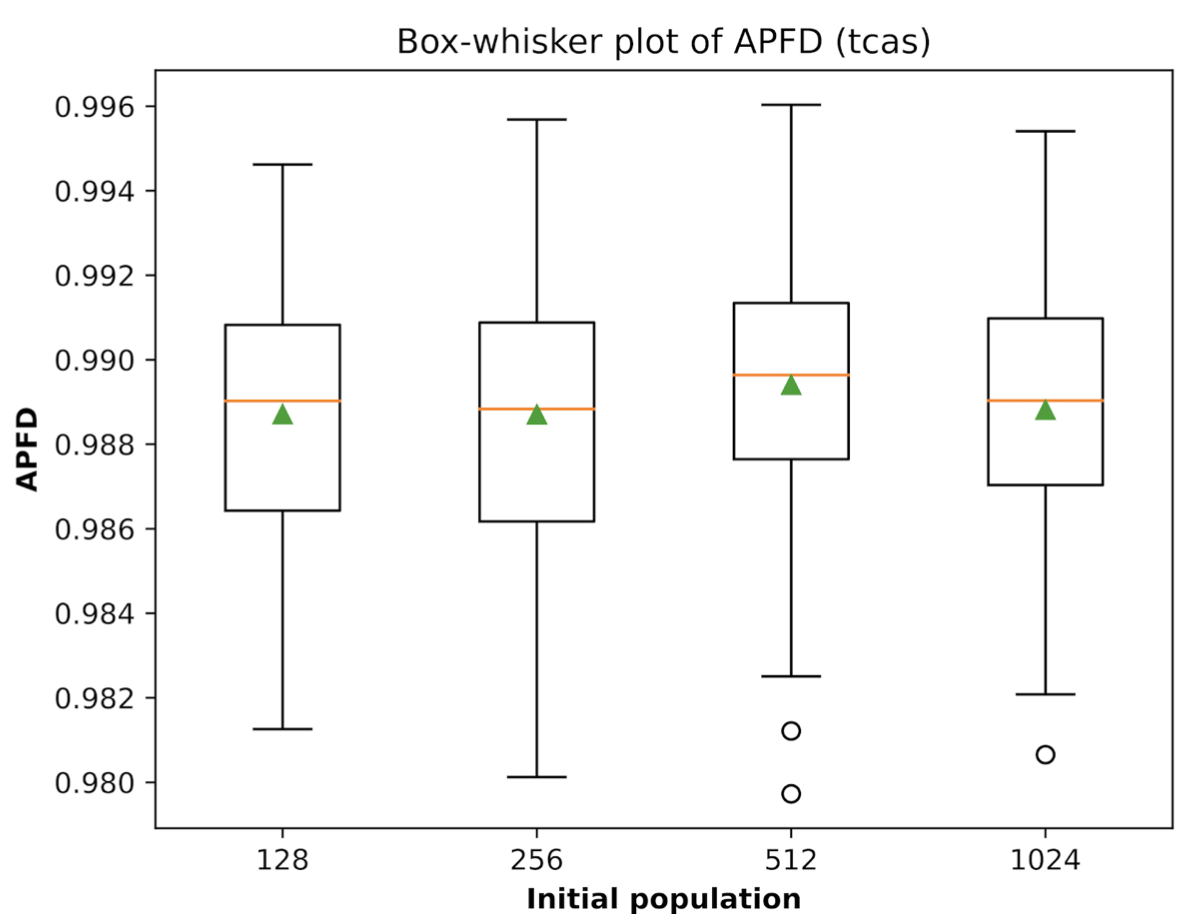
\includegraphics[width=\textwidth]{hyperparam/apfd.png}
			\caption{APFD}
		\end{subfigure}
		\caption{Effect of hyperparameters(initial population) on APSD and APFD, for tcas.}
		\label{fig:hyperparam}
	\end{figure*}
	
	\subsection{Embedding Scheme}
	\label{sec:embedding}
	\subsubsection{Overview}
	Let us recall some concepts from combinatorics and polytope theory:
	
	\begin{definition}
		For fixed $n$, the {\bf permutahedron}, denoted as $\Pi_{n-1}$, is defined as the convex hull of the set $S = \{ (\pi(1), \dots, \pi(n)) \ | \ \pi \in S_n \}$. 
	\end{definition}
	
	Permutahedron, first introduced in \cite{permutahedron}, has been a subject of intensive study in the field of not only combinatorics, but also in other fields such as bandit optimization\cite{bandit}, .
	We shall look at two important properties of $\Pi_{n-1}$ and their implications in our current problem. Refer to \cite{polytope, combinatorics} for the full proofs and more detailed discussions on related topics.
	
	\begin{lemma}
		$\Pi_{n-1}$ is a simple polytope of dimension $n - 1$, with $n!$ vertices given as $S$.
	\end{lemma}
	
	This shows that directly embedding $S$ onto $\mathbb{R}^n$.
	
	\begin{lemma}
		$\Pi_{n-1}$ is a geometric realization of weak Bruhat order on $S_n$ i.e. two vertices of $\Pi_{n-1}$ are adjacent iff they differ by a swap.
	\end{lemma}
	
	Above lemma has the important implication that {\it such simple and intuitive geometric realization(embedding) of $S_n$ onto $\mathbb{R}^{n-1}$ (with the usual Euclidean metric) has a very mathematically desirable structure}.
	In other words, this motivates for us to {\bf directly use continuous SWAY\cite{SWAY}}!
	
	\subsubsection{Mathematical Justification}
	However, it is not clear at first of how the $l2$-norm of two permutations is related to their swap distance.
	It may be that even though two permutations are far apart in $\mathbb{R}^{n-1}$ in $l2$-distance, they may be similar in swap distance or vice versa.
	In this subsection, we provide a mathematical justification that such case is not possible, in general.
	
	To see this, we need some concepts from statistical ranking theory:
	\begin{definition}
		{\bf Spearman $\rho$ distance} of $\pi, \pi' \in S_n$, denoted as $d_S(\pi, \pi')$, is precisely the Euclidean distance between $\pi$ and $\pi'$, considering them as vectors (vertices of $\Pi_{n-1}$ in $\mathbb{R}^n$)
	\end{definition}
	
	\begin{definition}
		{\bf Daniels-Guilbaud semi-metric}\footnote{Semi-metric is a generalized metric that doesn't satisfy the triangle inequality.} (abbreviated as DG-distance) of $\pi, \pi' \in S_n$, denoted as $d_G(\pi, \pi')$, is defined as the number of triples $(i, j, k), \ 1 \leq i < j < k \leq n$ such that $(\pi_i, \pi_j, \pi_k)$ is not a cyclic shift of $(\pi_i', \pi_j', \pi_k')$.
	\end{definition}
	
	\begin{definition}
		$\pi, \pi' \in S_n$ are said to have a {\bf circular agreement} on $\{x, y, z\} \subset [n]$ if $(\pi_x, \pi_y, \pi_z)$ can be obtained via a circular permutation of $(\pi'_x, \pi'_y, \pi'_z)$.
	\end{definition}
	
	The following results from \cite{Monjardet98} provide a key theoretical characterization of our approach\footnote{In our final presentation video, we claimed that there was an elegant statistical characterization of $d_G(\cdot, \cdot)$ and deferred the proof to here. However, after a careful scrutinization, we realized that there was a significant flaw in the proof, thus forcing us to remove the ``result". Still, we provide an equally elegant theoretical explanation for our embedding, although only based on existing results.}:
	\begin{theorem}[Monjardet, 1998]
		\[ d_S^2(\pi, \pi') = n d_K(\pi, \pi') - d_G(\pi, \pi') \quad \forall \pi, \pi' \in S_n \]
	\end{theorem}
	
	\begin{lemma}[Monjardet, 1998]
		\[ d_G(\pi, \pi') + a_G(\pi, \pi') = \binom{n}{3} \]
	\end{lemma}
	
	Here, $a_G(\pi, \pi')$ is defined as the number of triplets $\{x, y, z\} \in [n]$ such that $\pi$ and $\pi'$ have a circular agreement on.
	(Basically, it can be thought of as a ``dual" to $d_G$)
	
	Writing it in another way, 
	\[ d_S^2(\pi, \pi') = n d_K(\pi, \pi') + a_G(\pi, \pi') - \binom{n}{3} \]
	
	One can thus say that $\pi, \pi'$ are far apart in $\mathbb{R}^n$ if 
	\begin{enumerate}
		\item $d_K(\pi, \pi')$ is large i.e. they differ by a lot of swaps.
		\item $a_G(\pi, \pi')$ is large i.e. they are quite mixed up.
	\end{enumerate}
	
	Based on these mathematically rigorous results, we argue that our embedding, up to some level of distortion, accurately model the swap distance of two permutations, and thus it is okay to use the continuous version of SPLIT for our problem.
	
	
	\subsection{Initial population}
	For small $n$, using all of $S_n$ is not so much of a problem.
	However, it becomes a big problem when $n$ is big, especially in many of the industrial cases.
	Using all of $S_n$ for initialization requires $n!$ points, multiplied by the space complexity required for used embedding scheme.
	
	Thus we propose generating $2^k$ random permutations from $S_n$.
	Such sampling is done using Fisher-Yates shuffle, which outputs uniformly distributed permutations\cite{}({\bf CITATION}).
	We use Python's \textsc{random.shuffle} function, which makes use of the Fisher-Yates algorithm.
	
	
	\subsection{\textsc{Better} function}\label{sec:better}
	Using the already-known execution information of each test case, we've used APSD\cite{RYCC01} as our \textsc{Better} function, given as
	\begin{equation}
		\label{eq:apsd}
		APSD(T) = 1 - \frac{TS_1 + \dots + TS_m}{nm} + \frac{1}{2n}
	\end{equation}
	
	where $TS_i$ is the index of the first test case that covers statement $i$, $n$ is the number of test cases in the test suite, and $m$ is the number of statements in the program. 
	Such choice is natural since our current approach is coverage-based, and APSD is the most widely used function for measuring the early coverage percentage.
	
	
	
	\section{Experiments}
	
	\subsection{Benchmarks}
	Software-artifact Infrastructure Repository (SIR)\cite{sir} is an infrastructure, created to support controlled experimentation with testing techniques. It is home to many software-related artifacts that support rigorous controlled experimentation with program analysis and software testing techniques. 
	
	We consider $6$ Siemens programs, introduced by the Siemens Corporate Research for a study of the fault detection capabilities of control-flow and data-flow coverage criteria\cite{siemens}.
	Those programs were developed to study the fault detection of the code. This programs perform a variety of tasks (also referred to as programs): {\bf schedule, schedule2, printtokens, printtokens2, tcas, totinfo}. For each programs, it contains large pool of test cases.
	
	Below is a brief description of each program:
	\begin{enumerate}
		\item {\bf schedule, schedule2}: priority schedulers.
		
		\item {\bf printtokens, printtokens2}: lexical analysers
		
		\item {\bf tcas}: an aircraft collision avoidance system.
		
		\item {\bf totinfo}: computes statistics of given input data.
	\end{enumerate}
	
	Refer to \cite{siemens} for a detailed explanation on how the programs were seeded with faults, and how the test suites were made.
	For our experiment, we considered the $1000$ test suites in the folder {\it tesplans-bigcov}; those of which are suspected to have large sizes with full coverage.
	
	
	\subsection{Research Questions}
	To explore our approach of applying SWAY to TCP, we organize our exploration around the following research questions (RQ):
	\begin{enumerate}
		\item {\bf (RQ1)} How well SWAY performs compared to the state-of-the-art method for TCP?
		\item {\bf (RQ2)} How sensitive is SWAY to the initial population? (which is practically the only hyperparameter)
	\end{enumerate}
	
	As mentioned in Section \ref{sec:existing}, we only consider additional greedy algorithm as our competitor since it is simple to implement, and it shows comparable performance with the other search-based algorithms.
	In addition, for sanity check, we've also considered random algorithm, which just outputs a random permutation.
	For each program, a boxplot of APSD and APFD is plotted for each algorithm, where all $1000$ test suites were considered.
	
	\subsection{Performance Measures}
	We had used two metrics for the performance measure of SWAY and the compared existing methods. 
	
	The first metric is Average Percentage of Statement Detection(APSD). It measures how early the test suite can cover the whole statements of the given program. Since SWAY took coverage-based approach for TCP, we measured and compared APSD for the results of each method to see if SWAY had worked properly as it was expected. Its formula is given in Eq. \ref{eq:apsd}.
	
	The second metric we had used is Average Percentage of Fault Detection(APFD), which is a widely used performance metric for TCP problems. It measures how early the test suite can detect the faults of the whole program, which accords with the goal of TCP. APFD is given as
	\[ APFD(T) = 1 - \frac{TF_1 + \dots + TF_m}{nm} + \frac{1}{2n} \]
	
	where $TF_i$ is the index of the first test case that detects fault $i$, $n$ is the number of test cases in the test suite, and $m$ is the number of faults in the program. 
	
	
	
	\section{Results}
	All our codes are available in our Github repository\footnote{\url{https://github.com/Dongmin1215/CS454_Team5}}.
	
	\subsection{RQ1: How well does our approach perform?}
	Figures \ref{fig:main1}, \ref{fig:main2}, \ref{fig:main3} show the resulting box-plots of all the programs considered.
	Green triangle is the mean of the metric considered.
	For simplicity, additional greedy algorithm is labeled as ``greedy".
	
	As for APSD, all three algorithms considered did not show a significant difference among all the programs considered.
	Although there are some programs in which SWAY was outperformed by the additional greedy algorithm, it can be seen that SWAY performs comparably with the additional greedy algorithm.
	Note that in general, observing the number of outliers and the location of quartiles, it can be claimed that SWAY has less variance than random and additional greedy algorithm, showing that SWAY-based approach is more robust to different test suites.
	Similar trend is observed for APFD, although not as clear as APSD since we're directly optimizing over APSD.
	
	As an additional observation, note that there are some programs in which a uniformly randomly chosen permutation performs comparably with both additional greedy algorithm and SWAY (e.g. {\bf schedule}).
	We suspect that this is due to the excessively simple structure of the faults seeded in the programs, and thus the difference between different test cases orderings is very subtle.
	
	
	\subsection{RQ2: Sensitivity of hyperparameters}
	For the sake of simple exposition, we did this experiment with the {\bf tcas} program, only. However, we suspect that similar results will show up for other Siemens programs.
	We considered the initial population of $\{128, 256, 512, 1024\}$. As one can observe in Figure \ref{fig:hyperparam}, the results do not show a big difference.
	This is a rather surprising, yet desirable, result since it implies that our algorithm is very robust to the initial population (despite the intuition that more initial population leads to larger searches and thus better performance).
	However, since this is only for the Siemens programs, future research should explore whether this holds for other (more complex) programs, such as {\bf space}\cite{space}.
	
	
	\section{Conclusions and Future Work}
	In this paper, we propose a novel way of applying SWAY, a  baseline optimizer for multi-objective software engineering problems, to TCP (and possibly other problems whose decision space is the space of permutations).
	Specifically, we adopted the embedding of the permutations into the Euclidean space, and set the \textsc{Better} function as APSD which let the algorithm take coverage-based approach of TCP.
	We provide rigorous contextual evidence from well-established fields such as combinatorics, polytope theory, and statistical ranking theory to show that our embedding scheme is suitable for the framework of SWAY.
	
	In RQ1, we verified our algorithm by comparing it with random permutations and the widely used additional greedy algorithm, for the Siemens programs. Both in terms of APSD and APFD, SWAY performed comparably with additional greedy algorithm. For some programs, SWAY is more robust in terms of different test suites.
	In RQ2, we observed that initial population size didn't have much impact on the performance of SWAY for {\bf tcas} program, although we suspect that this would be the case for other programs as well.
	Additionally, we observe that random permutation is at par with additional greedy algorithm and SWAY for some of the Siemens programs, hinting that they might not be suitable for future research on test case prioritisation.
	
	One immediate direction for extending this work is to try another embedding, as described in Appendix \ref{sec:appendix}.
	This embedding exactly preserves the swap distance between two permutations, without any distortion, but at the cost of higher computational complexity.
	Due to time constraint, we couldn't implement this strategy, and so it would be interesting to see if this strategy is effective.
	
	Another is to consider some variants of TCP:
	\begin{enumerate}
		\item Since SWAY was proposed as an alternative to multi-objective problem, it would be interesting to use the same embedding for more complex variants of TCP such as time-constrained prioritisation\cite{JP02, DMTR10}.
		
		\item Here, we've only considered the approach of considering the permutation as the decision space i.e. each embedded point is a distinct test suite.
		It would be interesting to see if it is possible (and if it is maybe better) to embed each test case as a point.
		This idea may be lead to a new algorithm when considering a diversity-based approach to TCP.
		
		\item TCP considered here is called {\it white-box execution-based prioritisation})\cite{THHBD14} because we assumed that we have access to the source code of the SUT, and that we could execute the test cases.
		It would be interesting to see how to apply SWAY in the opposite situation, often called {\it black-box static prioritisation}.
		\cite{LPBS09, LPBMN12, THHBD14} tackled this problem by using string embedding, of which the future algorithm may be benefited from.
	\end{enumerate}
	
	Although our work is only about TCP, it is straightforward to try applying our algorithm to other SBSE problems with decision space of permutations. Some examples are:
	\begin{itemize}
		\item Traveling salesman problem(TSP)
		
		\item Permutation flow shop scheduling problem
		
		\item Quadratic assignment
		
		\item Linear ordering
	\end{itemize}
	
	
	
	% use section* for acknowledgment
	\ifCLASSOPTIONcompsoc
	% The Computer Society usually uses the plural form
	\section*{Acknowledgments}
	\else
	% regular IEEE prefers the singular form
	\section*{Acknowledgment}
	\fi
	
	
	The authors would like to thank Prof. Shin Yoo and Seungmin Lee of COINSE Lab (KAIST) for their insightful advices and guidances.
	
	
	% Can use something like this to put references on a page
	% by themselves when using endfloat and the captionsoff option.
	\ifCLASSOPTIONcaptionsoff
	\newpage
	\fi
	
	
	
	% trigger a \newpage just before the given reference
	% number - used to balance the columns on the last page
	% adjust value as needed - may need to be readjusted if
	% the document is modified later
	%\IEEEtriggeratref{8}
	% The "triggered" command can be changed if desired:
	%\IEEEtriggercmd{\enlargethispage{-5in}}
	
	% references section
	
	% can use a bibliography generated by BibTeX as a .bbl file
	% BibTeX documentation can be easily obtained at:
	% http://mirror.ctan.org/biblio/bibtex/contrib/doc/
	% The IEEEtran BibTeX style support page is at:
	% http://www.michaelshell.org/tex/bibtex/
	\bibliographystyle{IEEEtran}
	% argument is your BibTeX string definitions and bibliography database(s)
	\bibliography{_report}
	
	
		\appendices
	% you can choose not to have a title for an appendix
	% if you want by leaving the argument blank
	\section{Another Embedding}
	\label{sec:appendix}
	Let us recall an important concept from coding theory\cite{coding}:
	\begin{definition}
		Given any two vectors(codewords) $x = (x_1, \dots, x_n)$ and $y = (y_1, \dots, y_n)$, the {\bf Hamming distance} between $x, y$, denoted as $d_H(x, y)$, is defined as
		\[ d_H(x, y) := \sum_{i=1}^n \left[x_i \stackrel{?}{=} y_i\right] \]
		
		where $\left[x_i \stackrel{?}{=} y_i\right]$ is the indicator function of whether $x_i$ is equal to $y_i$.
		
		(The definition naturally extends for two equal-sized matrices by considering their vectorizations.)
	\end{definition}
	
	One can immediately see that if $x, y \in \{0, 1\}^n$, then $d_H(x, y)$ can be rewritten as $\sum_{i=1}^n |x_i - y_i|$ i.e. the {\it Jaccard distance} between $x$ and $y$.
	
	The following lemma from \cite{cormode} is the key theoretical basis for this embedding:
	\begin{lemma}
		\[ \forall \pi, \pi' \in S_n \quad d_K(\pi, \pi') = d_H \left( S(\pi), S(\pi') \right) \]
		
		where $[S(\pi)]_{ij} := [i < j \wedge \pi^{-1}(i) < \pi^{-1}(j)]$ and $[\cdot]$ is the indicator function for the given logical predicate.
	\end{lemma}
	
	The significance of above lemma is that {\it such binary embedding scheme gives a distortion-free embedding of $S_n$ onto $\{0, 1\}^n$ with Hamming distance as the endowed metric}\footnote{This space is known as the {\it Hamming space} in coding theory.} i.e. we can {\bf directly use binary SWAY} as proposed in \cite{SWAY}!
	Moreover, note that in our binary case, the Hamming distance is equivalent to the Jaccard distance, providing further justification for the direct application of binary SWAY.
	
	Lastly, noting that for all $\pi \in S_n$, $S(\pi)$ is anti-symmetric (if $(i, j)$-th component is $1$, then $(j, i)$-th component is $0$ and $(i, i)$-th component is $0$), we can reduce the space complexity from $n^2$ to $\frac{n(n-1)}{2}$.
	
	Note that in exchange for preserving the pairwise swap distances, the space complexity (and thus the expected computational complexity) is rather high.
	It takes $O(N_0 n^2)$ space complexity with $O(N_0 n)$ time complexity for embedding each permutation, where $N_0$ is the size of the initial population.
	Our embedding scheme as mentioned in Section \ref{sec:embedding} takes $O(N_0 n)$ space complexity with $O(N_0)$ time complexity for embedding each permutation, but at the cost of some distortion introduced.
	Thus there is a clear trade-off between the two embedding schemes, and it would be interesting to see if such trade-off extends to performance of the algorithm.
	
	% that's all folks
\end{document}


